%% Adaptive and Cost-Aware Data Quality Monitoring for Evolving Data Pipelines
%% Target venue: ACM Journal of Data and Information Quality (JDIQ), acmart / acmsmall.
%% Format follows the official "ACM Journals Primary Article Template" on Overleaf.
%% JDIQ is an ACM journal, so it uses the single-column journal layout and the Libertine typeface
%% (two-column "sigconf" is the ACM conference-proceedings layout, not the journal layout).
%%   Submission for review (what the template requires):   \documentclass[manuscript,screen,review]{acmart}
%%   Double-anonymous review, if the journal asks for it:   \documentclass[manuscript,screen,review,anonymous]{acmart}
%%   Published journal look (acmsmall, for proofreading):  \documentclass[acmsmall,screen]{acmart}
\documentclass[manuscript,screen,review]{acmart}

\usepackage{booktabs}
\usepackage{tabularx}
\usepackage{multirow}
\usepackage{siunitx}
\usepackage{tikz}
\usetikzlibrary{arrows.meta,positioning,fit,backgrounds}
\sisetup{group-separator={,},group-minimum-digits=4}
\setlength{\emergencystretch}{2em}

\setcopyright{none}
\settopmatter{printacmref=false}
\acmJournal{JDIQ}
\acmYear{2026}
\acmVolume{1}
\acmNumber{1}
\acmArticle{1}
\acmMonth{10}

\newcommand{\pp}{\,pp}
\makeatletter
\newcommand\inputtable[1]{\@@input #1 }
\makeatother

\begin{document}

\title{Adaptive and Cost-Aware Data Quality Monitoring for Evolving Data Pipelines}
\subtitle{Separating Legitimate Drift from Degradation under a Frozen Evaluation Protocol}

\author{Muzakkiruddin Ahmed Mohammed}
\authornote{Both authors contributed equally to this research.}
\email{mmohammed6@ualr.edu}
\affiliation{%
  \institution{University of Arkansas at Little Rock}
  \city{Little Rock}
  \state{Arkansas}
  \country{USA}}

\author{Ahsan Shahid}
\authornotemark[2]
\email{axshahid@ualr.edu}
\affiliation{%
  \institution{University of Arkansas at Little Rock}
  \city{Little Rock}
  \state{Arkansas}
  \country{USA}}

\author{Selimhan Dagtas}
\email{sedagtas@ualr.edu}
\affiliation{%
  \institution{University of Arkansas at Little Rock}
  \city{Little Rock}
  \state{Arkansas}
  \country{USA}}

\author{John Talburt}
\email{jrtalburt@ualr.edu}
\affiliation{%
  \institution{University of Arkansas at Little Rock}
  \city{Little Rock}
  \state{Arkansas}
  \country{USA}}

\author{Abdelrahman Elfikky}
\email{aelfikky1@ualr.edu}
\affiliation{%
  \institution{University of Arkansas at Little Rock}
  \city{Little Rock}
  \state{Arkansas}
  \country{USA}}

\renewcommand{\shortauthors}{Mohammed et al.}

\begin{abstract}
Data quality rules in recurring batch pipelines must accommodate legitimate change without accepting persistent errors as normal. Fixed thresholds can raise false alarms under distribution drift, whereas unrestricted adaptation can weaken error detection. This article presents and evaluates an adaptive and cost-aware monitoring framework that combines numerical threshold adaptation, gated drift estimation, historical admission of large language model (LLM) rules, guarded category learning, and risk-based check selection. Separate drift and failure signals assign each batch one of four labels: stable, drift, degradation, or drift with degradation. Evaluation uses three public datasets, seventeen controlled scenarios, and ten paired test seeds under an internally frozen protocol, supplemented by two error-labelled benchmarks and a sixteen-year chronological replay. Four-class macro-F1 ranges from 0.947 to 0.966, although the same gate with fixed thresholds performs comparably on two datasets. Adaptation reduces drift-related false positives on flight data but loses up to 29 percentage points of recall under persistent contamination; its false-positive criterion is not supported on retail data. Fixed statistical rules combined with admitted LLM rules achieve 99.6--100\% recall on injected domain-impossible values. A separate per-value category check admits all twelve valid novel values and rejects eleven of twelve invalid values. Risk-based selection saves 2--11\% of checks, but provides little total runtime benefit after profile statistics are reused. The findings identify where adaptation, domain knowledge, and selective execution contribute to monitoring quality, and the conditions that limit those contributions.
\end{abstract}


%% CCS concepts: generate the CCSXML block at https://dl.acm.org/ccs before submission.
\ccsdesc[500]{Information systems~Data cleaning}
\ccsdesc[300]{Information systems~Extraction, transformation and loading}
\ccsdesc[300]{Computing methodologies~Anomaly detection}

\keywords{data quality monitoring, data validation, concept drift, adaptive thresholds, large language models, rule generation, risk-based validation, data pipelines}

\maketitle

\section{Introduction}
\label{sec:intro}

Data pipelines repeatedly collect, transform, and deliver records for analysis and operational decisions. A pipeline may load flight records each day, invoice lines each hour, or inspection outcomes each month. Declarative quality rules guard these batches by checking properties such as completeness, uniqueness, numerical plausibility, and membership in a valid category domain. Systems including Deequ~\cite{Schelter2018,Schelter2019}, TensorFlow Data Validation (TFDV)~\cite{Breck2019,Caveness2020}, and Data Sentinel~\cite{Swami2020} make such checks repeatable and support profiling or constraint management. Their effectiveness nevertheless depends on how validation expectations are established and maintained as the data change.

Three connected difficulties motivate this study. First, a fixed expectation can become outdated even when the pipeline is working correctly. Seasonal demand, congestion, and revised reporting procedures can alter valid values, causing rules learned from an earlier sample to reject later records. In the flight-data experiment, a mean-plus-or-minus-three-standard-deviations rule calibrated on five warm-up batches flags approximately 4.6\% of valid records at 2\% injected drift and 7.6\% at 30\% drift, despite an unchanged 1\% background error rate. A growing alarm rate can therefore reflect legitimate evolution rather than deteriorating quality.

Second, learning from recent batches can create the opposite problem. An adaptive range may follow valid changes in location and scale, but it may also widen around recurring numerical corruption. Likewise, repeated observation of a previously unseen country name does not establish that the name is valid: the value may be a persistent misspelling. A monitor must balance responsiveness to change against preservation of the constraints that define errors. Reducing the number of alarms alone is not evidence that this balance has been achieved.

Third, validation consumes resources. Executing every check on every batch can repeat scans and spend effort on columns that show little evidence of change. Risk-based validation proposes directing effort toward the probability and consequence of data problems~\cite{FoidlFelderer2019}. Its practical value, however, depends on whether selection preserves detection and whether skipped checks represent a substantial share of total monitoring work. Profiling and drift estimation may remain necessary even when some checks are omitted.

These difficulties also affect the interpretation of an alarm. An operator needs to know whether a batch differs from history because valid data have changed, because errors have increased, or because both occurred. We refer to legitimate distribution change as \emph{drift} and increased erroneous-record prevalence as \emph{degradation}. These properties are distinct but can coexist. A distribution-change signal alone cannot explain which condition holds; a rule-failure signal alone can mistake outdated expectations for poor quality. The framework therefore combines the two signals while retaining separate measurements of record-level detection and batch-level classification.

Relevant research supplies several of the necessary building blocks. History-aware validation learns expectations from recurring pipeline executions~\cite{Redyuk2021,Tu2023,Shankar2023}. Drift research provides methods for comparing distributions~\cite{Gama2014,Lu2019,Rabanser2019}. LLMs can translate schema descriptions, examples, and requirements into candidate quality conditions~\cite{Glock2026,Xie2025,Abughazala2026,Chen2026}. These developments motivate an integrated evaluation rather than an assumption that combining them necessarily improves performance. In particular, useful evidence must separate the contribution of threshold adaptation from that of drift gating, distinguish domain knowledge from historical frequency, and compare selective execution with simpler schedules at a similar check budget.

This article develops a configurable batch monitor to investigate those questions within one framework. It profiles each batch, constructs static and statistical checks, admits LLM and dictionary-only model proposals after warm-up validation, adapts numerical ranges, and selects checks through a per-column risk score. A gated distribution comparison and a failure-rate signal then assign one of four batch labels. Category-guard policies are evaluated separately to determine which forms of domain evidence can constrain the admission of recurring new values.

The evaluation addresses three research questions. RQ1 asks whether adaptive thresholds reduce false positives under legitimate drift without an unacceptable recall loss, and whether the combined signals distinguish the four batch conditions. RQ2 asks whether admitted LLM rules add coverage of domain-impossible values and whether domain checks improve category admission. RQ3 asks whether risk-based check selection reduces execution cost while maintaining detection after degradation begins. These objectives are evaluated individually, so that success of one component is not treated as success of every configuration.

Three public datasets cover transport, retail, and public health. Seventeen controlled scenarios provide audited injected-error labels, while disjoint development and test record pools separate method development from the paired test evaluation. The internally frozen protocol specifies the margins, settings, and ten test seeds. Comparators include pooled fixed, rolling, robust, and exponentially weighted thresholds; an AVH-inspired historical-statistics baseline~\cite{Tu2023}; and configured Deequ and TFDV runs. Two dirty/clean benchmark pairs~\cite{Mahdavi2019} and a chronological Chicago replay examine transfer beyond shuffled controlled batches.

The article makes the following contributions.
\begin{enumerate}
\item An integrated monitoring loop that combines gated drift evidence and rule-failure evidence to assign four operational batch labels, with warm-up drift calibration based on leave-one-out scoring and resampling (Section~\ref{sec:method}).
\item A paired evaluation protocol with disjoint development and test records, prespecified non-inferiority margins, seed-cluster uncertainty estimates, and manifests recording code and configuration fingerprints (Section~\ref{sec:design}).
\item Dataset- and scenario-specific evidence on numerical and categorical adaptation, including reductions in drift-related false positives and losses in detection when persistent errors enter learned expectations (Section~\ref{sec:results}).
\item Evaluation of LLM-proposed rules and their admission procedure, including complementary statistical coverage, deliberately faulty candidates, dictionary-only model comparisons, and category-domain checks.
\item A cost analysis that distinguishes executed checks, estimated bytes touched, and measured monitoring phases, with matched scheduling baselines and a profile-reuse configuration.
\end{enumerate}

The results support conditional benefits. Four-class macro-F1 reaches 0.966, 0.955, and 0.947 on the three datasets, but the same drift gate with fixed thresholds gives identical Chicago results and no detected disadvantage on Retail. Threshold adaptation meets the primary false-positive and recall criteria in six of nine flight scenarios and nine of nine Chicago scenarios; Chicago's small gain comes from category policy. It does not meet the false-positive criterion on Retail. Fixed statistical rules combined with admitted LLM rules reach semantic recall of 0.996--1.00, whereas recurring invalid codes remain a weakness of adaptive combinations. Risk-based execution meets the point-estimate usefulness criterion in eleven of eighteen degradation/incident cases, with small absolute savings and little timing benefit after profile reuse. These findings identify both the contribution and the operating limits of the proposed framework.

The article is organised as follows. Section~\ref{sec:related} reviews related work. Section~\ref{sec:problem} defines the setting and hypotheses. Section~\ref{sec:method} explains the monitor, and Section~\ref{sec:design} describes the evaluation. Section~\ref{sec:results} reports the hypothesis results, ablation, external checks, and sensitivity analysis. Sections~\ref{sec:discussion} and~\ref{sec:conclusion} discuss their implications and conclude.

\section{Background and Related Work}
\label{sec:related}

This study draws on six connected areas: declarative data validation, history-aware validation, error detection and constraint discovery, distribution drift, LLM-based rule generation, and risk-based validation. Each area supplies a different kind of evidence about an incoming batch. A schema expresses expected structure, history describes previously observed behaviour, and domain rules express conditions that need not be recoverable from frequencies alone. Table~\ref{tab:positioning} summarises how these ideas inform the three research questions.

\subsection{Quality Dimensions and Declarative Validation}

Data quality is usually understood in relation to an intended use, rather than as a single property of a table. Foundational work distinguishes dimensions including accuracy, completeness, consistency and representational suitability~\cite{WangStrong1996,Batini2009,FanGeerts2012}. A monitor operationalises a subset of these dimensions through executable conditions: required values must be present, records must satisfy a specified uniqueness requirement, and values must belong to an accepted type or domain. Passing these checks establishes compliance with the chosen conditions; it does not establish that every recorded fact is correct. A valid inspection-result code, for example, can still describe an inspection inaccurately.

Declarative validation separates such conditions from their physical execution. Deequ expresses constraints over Spark tables, translates the required measurements into aggregation queries, and supports incremental computation and anomaly detection over historical quality metrics~\cite{Schelter2018,Schelter2019}. Its constraint suggestions reduce initial authoring effort, while explicit constraints allow engineers to encode requirements that profiles cannot infer reliably. This distinction matters here because statistical expectations and physical limits have different reasons to change.

TFDV combines descriptive statistics, schema inference and anomaly reporting, including comparisons between training, serving or successive data spans~\cite{Breck2019,Caveness2020}. Its schema can be reviewed and refined as data evolve. Data Sentinel illustrates declarative validation at production scale~\cite{Swami2020}. Deequ and TFDV already provide temporal and distributional monitoring capabilities; our comparison concerns their evaluated configurations and calibration choices, rather than an assumption that these frameworks only execute fixed rules.

Tool surveys document differences in profiling, measurement and monitoring support~\cite{Ehrlinger2022}, while production-ML studies explain why validation is needed throughout a pipeline's lifecycle~\cite{Sculley2015,Breck2017,Polyzotis2018}. Within that broader setting, this paper asks how to adjust expectations and allocate checks while preserving the distinction between legitimate distribution change and increased rule violations.

\subsection{History-Aware Validation}

History-aware methods reduce the need to specify every expected property manually. Auto-Validate learns data-domain patterns for string columns using evidence from data lakes~\cite{SongHe2021}. Redyuk et al.\ represent batches by descriptive quality statistics and apply novelty detection to identify deviations from previously accepted partitions~\cite{Redyuk2021}. Their method also adapts to temporal changes, making it directly relevant to recurring ingestion. Shankar et al.\ study automatic and precise validation for machine-learning pipelines~\cite{Shankar2023}. Together, these approaches show that history can supply validation evidence when detailed domain specifications are unavailable.

Auto-Validate-by-History (AVH) is particularly close to the present work~\cite{Tu2023}. It derives constraints from historical pipeline statistics and selects a set that balances coverage of generated errors against a false-positive budget. Its formulation recognises that retaining every plausible constraint can create an unacceptable aggregate alert rate. The AVH-inspired comparator used here follows a narrower historical-statistics design: it does not reproduce the published constraint-selection optimiser. Its results therefore characterise that local baseline under our four-class task, rather than the full AVH system.

Historical learning depends on what the accepted history represents. Previous successful ingestion can be evidence of operational acceptability, but it is not an independent guarantee of correctness. If an error persists, a moving numerical range or a category set learned by recurrence may gradually accommodate it. Related observations in the data-poisoning literature show how contaminated observations can alter learned behaviour~\cite{Biggio2012,Steinhardt2017}; the persistence scenarios here do not require an adversarial source. RQ1 examines this dependence through fixed, rolling, robust, exponentially weighted and current-batch policies, with common replay inputs and explicit decision criteria.

\subsection{Error Detection and Constraint Discovery}

Error detection asks which records or cells violate the intended meaning of the data. Abedjan et al.\ show that detectors have different strengths across error families and that combining signals is important~\cite{Abedjan2016}. Raha configures multiple detection strategies using limited user supervision~\cite{Mahdavi2019}; Baran addresses correction using contextual representations and transfer learning~\cite{MahdaviAbedjan2020}; and HoloDetect learns error detectors from a small labelled set with data augmentation~\cite{Heidari2019}. Their supervision and output granularity differ from an unsupervised batch alarm, so their tasks should not be treated as interchangeable.

Constraint discovery supplies another source of evidence. Functional dependencies capture relationships such as one attribute determining another~\cite{Papenbrock2015}; conditional functional dependencies restrict relationships to relevant subsets~\cite{Fan2008}; and denial constraints express combinations of values that should not coexist~\cite{Chu2013}. Such relations can expose errors that single-column ranges and category lists cannot detect. A city and a postal code may each be individually valid while their combination is inconsistent. Ilyas and Chu provide a broader treatment of how these signals support data cleaning~\cite{IlyasChu2019}.

The connection here is twofold. First, the error-labelled Tax and Beers tables test whether monitoring rules transfer beyond the controlled injection process. They are datasets from the Raha benchmark collection, not evaluations of Raha itself. Second, the Tax experiment compares learned cross-column dependencies with structures proposed by an LLM. This separates the value of relational information from the source that proposes the rule. Since these benchmarks are replayed in shuffled batches, they assess error coverage and localisation rather than naturally occurring temporal drift.

\subsection{Drift Detection}

Concept-drift research studies changing data-generating processes and how detection or learning procedures should respond~\cite{Gama2014,Webb2016,Lu2019}. Adaptive-window methods compare observations over time~\cite{BifetGavalda2007}, while dataset-shift studies examine tests on features and representations~\cite{Rabanser2019}. Our monitor uses distribution distances on batch profiles: a quantile approximation related to Wasserstein distance for numerical columns~\cite{Ramdas2017}, and Jensen--Shannon divergence for categorical frequencies~\cite{Lin1991}.

Distance choice and calibration answer different questions. A distance quantifies how much observed distributions differ; a threshold determines when that difference warrants an indication. Statistical process control supplies established historical baselines, including exponentially weighted moments~\cite{Roberts1959}. Median absolute deviation and interquartile fences provide robust alternatives when means and standard deviations poorly describe skewed data~\cite{Leys2013,Tukey1977}. Comparing calibrated versions is important because an apparent advantage can otherwise arise from different initial flag rates rather than adaptation.

Distribution change does not, by itself, establish a quality decline. A valid seasonal shift and an upstream error can both alter a profile. A change preserving common summary statistics can also violate a domain condition. RQ1 therefore combines drift evidence with a separate rule-failure signal. The gate in Section~\ref{sec:method:drift} limits the influence of records that fail available checks before classification drift is scored. Its interpretation remains conditional on those checks: filtering is a practical separation mechanism, not proof that every retained observation is valid.

\subsection{Rule Generation with Large Language Models}

Foundation models have been investigated for data-wrangling tasks, including error detection and transformation~\cite{Narayan2022}. Recent work uses them to translate domain knowledge into executable validation conditions. These studies differ in what they supply to the model, how they verify proposals, and which outcomes define success.

LeDQeR generates candidate rules from observed dirty tuples in the syntax of an existing data quality tool, then filters them for execution, correctness, coverage and redundancy~\cite{Glock2026}. It is close to the proposal-and-admission design considered here. The distinction is the evidence available to admission: our controlled-experiment candidates use descriptions and development examples, and are screened on a run's historical batches. A low historical flag rate establishes compatibility with those batches, rather than an independent correctness label.

LLM-DQR combines database schemas, natural-language requirements and sample records to generate rules for electronic health records~\cite{Xie2025}. Its validation loop includes deduplication, sandbox execution and iterative debugging. The study illustrates the value of domain context for complex rule construction, while its clinical coverage measures are not directly comparable with our record-level FPR or injected semantic recall. Quality by Prompt translates stated requirements into Great Expectations rules using a fine-tuned model~\cite{Abughazala2026}. Its focus on requirement translation differs from discovering missing constraints from historical data.

PrismaDV conditions test generation on downstream program code and dataset profiles, and uses task and test outcomes to adapt prompts through SIFTA~\cite{Chen2026}. It therefore already studies adaptive, task-aware validation. Our work examines a different mechanism: changing numerical ranges and category membership without downstream-task outcome supervision. SPADE synthesises and filters assertions using prompt-version histories and labelled outputs of LLM pipelines~\cite{Shankar2024SPADE}. Its assertion-selection problem is relevant to admission redundancy and coverage, although its generated-output setting differs from the tabular input batches evaluated here.

These studies establish that model proposals require execution and validation evidence. RQ2 builds on this premise by testing the additional coverage of admitted rules, the admission screen, and category-domain judgements. It distinguishes the ability to suggest a useful constraint from the ability to preserve that constraint while learning from later batches. Offline rule generation and per-value category checking are also separate configurations; success in one does not establish the performance of the other.

\subsection{Risk-Based Validation}

Risk-based validation directs effort toward data problems with greater likelihood or downstream impact~\cite{FoidlFelderer2019}. This motivates using observed failures, distribution changes and field importance to decide which checks deserve immediate execution. RQ3 turns that principle into an evaluated scheduling policy and compares it with periodic and random schedules at matched standard-check execution rates.

Selective execution and efficient execution address different costs. Sharing or incrementally computing metrics reduces work required by a check~\cite{Schelter2018}; scheduling avoids some checks altogether. A monitor that profiles every batch may retain substantial overhead even when optional checks are skipped. Accordingly, this study reports check counts, estimated bytes touched and phase-level runtime, including reuse of profile statistics. It also measures missed incidents, since a skipped check can withhold the evidence needed to raise its own future risk.

\subsection{Positioning}

The paper retains a focused objective: adaptive and cost-aware quality monitoring for evolving batch pipelines. Its components draw on established validation, drift and rule-generation ideas. The contribution lies in evaluating their behaviour together and separately under a common protocol, including conditions where benefits do not transfer. RQ1 tests adaptation and four-class labelling; RQ2 tests domain-rule coverage and category admission; and RQ3 tests the detection--cost trade-off. This positioning does not require a claim that earlier systems lack adaptation or that proposal filtering is itself new.

\begin{table}[t]
\caption{Position of this study relative to prior work. The third column identifies the connection examined here, rather than asserting that an entire research area has not addressed it.}
\label{tab:positioning}
\small
\begin{tabularx}{\linewidth}{@{}p{0.2\linewidth}p{0.24\linewidth}XX@{}}
\toprule
Line of work & Representative work & Connection to this study & Evaluated component \\
\midrule
Declarative validation & Deequ, TFDV, Data Sentinel & Explicit constraints and calibrated temporal comparisons & Rule execution; configured tool baselines \\
History-aware validation & Auto-Validate, Redyuk et al., Shankar et al., AVH & Expectations learned from recurring batches & Threshold policies; AVH-inspired baseline \\
Error detection and constraint discovery & Raha, Baran, HoloDetect, FD and CFD discovery & Complementary error signals and relational consistency & Error-labelled benchmarks; cross-column rules \\
Drift detection & Gama et al., Lu et al., Rabanser et al. & Distribution change and its distinction from rule failure & Gated drift; four batch labels \\
LLM rule generation & LeDQeR, LLM-DQR, Quality by Prompt, PrismaDV, SPADE & Candidate generation, filtering and domain context & Admission; semantic coverage; category guard \\
Risk-based validation & Foidl and Felderer & Prioritising validation effort and accounting for overhead & Risk score; matched schedules; phase timing \\
\bottomrule
\end{tabularx}
\end{table}


\section{Problem Formulation and Hypotheses}
\label{sec:problem}

\subsection{Setting and Definitions}

A pipeline delivers a sequence of batches $B_1, B_2, \ldots, B_T$ of records with a fixed schema. Each monitored column is either numerical or categorical. The first $w$ batches form a warm-up period that is assumed to be mostly clean; the monitor uses them to calibrate its rules and thresholds and does not report on them. In the experiments $T = 20$ and $w = 5$, and batches $B_6$ to $B_{20}$ are evaluated.

A record is \emph{erroneous} when at least one of its monitored values violates the intended meaning of the data: a value is missing, the record duplicates another, a categorical value lies outside the valid domain, or a numerical value is implausible or impossible in the domain. A monitor flags records; a flagged valid record is a false positive and an unflagged erroneous record is a false negative. These outcomes are evaluated against the injected-error answer key in controlled runs and the dirty/clean comparison convention in external benchmarks. A rule failure is evidence of a possible error, rather than an independent guarantee that the source value is factually incorrect.

A batch exhibits \emph{drift} when the distribution of its valid values differs from that of the warm-up because of a legitimate change in the world, such as longer taxi times during congestion or a new mix of inspection outcomes after a change of procedure. A batch exhibits \emph{degradation} when it contains more erroneous records than the warm-up did. In the controlled scenarios both properties are known by construction: a batch is a drift batch when its injected drift level is positive, and a degradation batch when its rate of erroneous records exceeds the warm-up rate for any reason, including incidents, sustained contamination, domain-impossible values and recurring invalid categories. A stable batch can still contain the unchanged background error rate; stable does not mean error-free. Every evaluated batch therefore carries one of four labels: \emph{stable}, \emph{drift}, \emph{degradation}, or \emph{drift with degradation}.

The monitor has two tasks per batch. At record level it flags erroneous records. At batch level it assigns one of the four labels. It also decides, before executing any check, which checks to run. These decisions have different purposes: record flags locate suspected problems, batch labels support operational interpretation, and selection allocates execution effort. They are measured separately because a good result on one task does not establish a good result on the others.

The distinction between drift and degradation is known by construction in controlled scenarios. During natural operation, the monitor instead infers them from distribution comparisons and detected failures. Its labels are consequently operational estimates conditional on the rules, reference data, and checks available, not causal proof of why the data changed.

\subsection{Research Questions and Hypotheses}

\paragraph{RQ1: Adaptation under drift.} Do adaptive thresholds handle legitimate drift better than fixed and history-based thresholds, and can the monitor separate drift from degradation?

\begin{itemize}
\item \textbf{H1a.} In each dataset and scenario, adaptive thresholds have a lower record-level false-positive rate (FPR) than fixed thresholds computed on the pooled warm-up, and their recall is non-inferior within a margin of 1 percentage point. The scenarios of interest are those with drift; scenarios without drift test whether adaptation costs anything when nothing changes.
\item \textbf{H1b.} A gated drift signal combined with a failure-rate signal assigns the four batch labels with a higher macro-averaged F1 than the comparators, which include the same drift signal paired with non-adaptive thresholds, the same monitor without the gate, and established tools.
\end{itemize}

\paragraph{RQ2: Domain knowledge from rules.} Do validated LLM rules add coverage that statistical rules lack, and can domain constraints stop the monitor from learning invalid values?

\begin{itemize}
\item \textbf{H2a.} On domain-impossible values that are statistically unremarkable, statistical rules combined with validated LLM rules reach higher recall than either rule source alone, while the FPR rises by no more than 0.5 percentage points.
\item \textbf{H2b.} When new categories may be learned only if they are compatible with independently justified domain constraints, recurring invalid categories are admitted less often than under learning by recurrence alone, while valid new categories are still admitted.
\end{itemize}

\paragraph{RQ3: Cost.} Can risk-based selection of checks reduce the cost of monitoring without a large loss in detection?

\begin{itemize}
\item \textbf{H3.} In scenarios with sustained degradation or incidents, selecting checks by a per-column risk score executes fewer checks than running every check, while recall on the records after the onset of the problem stays at or above 0.90. A configuration that meets both conditions is called \emph{useful}. Risk-based selection should be useful more often than periodic or random selection that executes the same number of checks.
\end{itemize}

\subsection{Prespecified Decision Criteria}

The decision thresholds were specified in the internally frozen protocol and are retained for the test evaluation. The margins express the required trade-offs rather than quantities optimised after observing the results. The recall non-inferiority margin is 1 percentage point. The argument for this value has three parts. First, the comparators detect about 99.5 to 100\% of the injected errors in the stable scenario, and a 2-point margin would allow up to five times as many missed errors. Second, at a 1\% error rate one point of recall corresponds to one additional missed error per 10,000 records, against the 200 to 440 fewer false alarms per 10,000 valid records that adaptation produced under drift in a preliminary study. Third, ten paired seeds were expected to give confidence intervals for a pooled recall difference a few tenths of a point wide, narrow enough to decide a 1-point margin. (On the retail data the intervals turned out wider; Section~\ref{sec:res:h1a} reports them.) The tolerated rise in FPR for H2a is 0.5 percentage points. The detection target for H3 is a post-onset recall of 0.90. All intervals are 95\% intervals. H1a decisions are made per dataset and scenario using paired confidence bounds. H3 usefulness is assessed from the reported mean recall and positive check saving; it does not require the lower confidence bound to exceed 0.90. Secondary comparator comparisons use the Holm procedure~\cite{Holm1979}; the reporting correction and its family definition are explained in Section~\ref{sec:design}. These criteria are not a claim of study-wide superiority across every dataset, scenario, and metric.

\section{Monitoring Method}
\label{sec:method}

The framework processes each batch through profiling, rule construction, selection, execution, classification, and persistence (Figure~\ref{fig:loop}). Raw profile drift is available before selection and contributes to the risk score. After the selected checks run, their evidence supports gated drift estimation and batch labelling. These are two related drift calculations with different information available to them; the classifier's gated signal is not assumed to exist before check execution.

Each monitoring phase is timed separately for the cost analysis in Section~\ref{sec:res:h3}. Warm-up calibration establishes the initial reference and failure baselines. Thereafter, the monitor updates state after each batch. The numerical adaptation, category policies, and scheduler settings described below are those used in the frozen evaluation.

\begin{figure}[t]
\centering
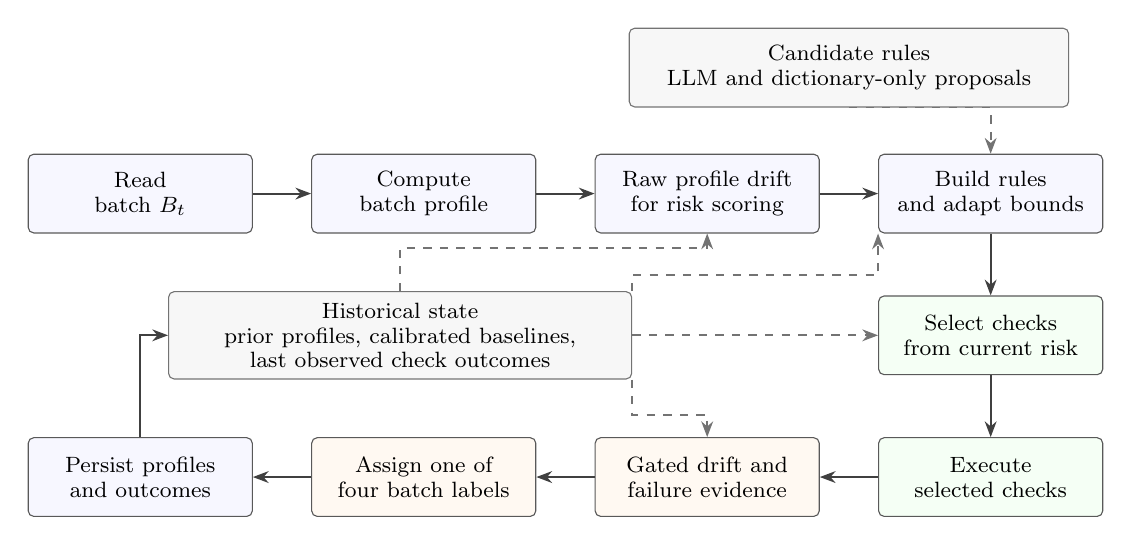
\begin{tikzpicture}[
  x=1cm,y=1cm,
  box/.style={draw=black!65,rounded corners=2pt,align=center,
    font=\fontsize{8}{9}\selectfont,minimum height=10mm,text width=26mm,
    inner sep=3.5pt,fill=blue!3},
  store/.style={draw=black!55,rounded corners=2pt,align=center,
    font=\fontsize{8}{9}\selectfont,minimum height=10mm,inner sep=4pt,fill=black!3},
  arr/.style={-{Stealth[length=2mm]},line width=.7pt,draw=black!75},
  state/.style={arr,dashed,draw=black!55}]
\node[box] (read) at (0,0) {Read\\batch $B_t$};
\node[box] (prof) at (3.6,0) {Compute\\batch profile};
\node[box] (raw) at (7.2,0) {Raw profile drift\\for risk scoring};
\node[box] (build) at (10.8,0) {Build rules\\and adapt bounds};
\node[box,fill=green!4] (select) at (10.8,-1.8) {Select checks\\from current risk};
\node[box,fill=green!4] (execute) at (10.8,-3.6) {Execute\\selected checks};
\node[box,fill=orange!5] (gate) at (7.2,-3.6) {Gated drift and\\failure evidence};
\node[box,fill=orange!5] (label) at (3.6,-3.6) {Assign one of\\four batch labels};
\node[box] (persist) at (0,-3.6) {Persist profiles\\and outcomes};
\node[store,text width=56mm] (history) at (3.3,-1.8)
  {Historical state\\prior profiles, calibrated baselines,\\last observed check outcomes};
\node[store,text width=53mm] (candidates) at (9.0,1.6)
  {Candidate rules\\LLM and dictionary-only proposals};
\draw[arr] (read)--(prof);
\draw[arr] (prof)--(raw);
\draw[arr] (raw)--(build);
\draw[arr] (build)--(select);
\draw[arr] (select)--(execute);
\draw[arr] (execute)--(gate);
\draw[arr] (gate)--(label);
\draw[arr] (label)--(persist);
\draw[arr] (persist.north) |- (history.west);
\draw[state] (candidates.south) -| (build.north);
\draw[state] (history.north) -- ++(0,.55) -| (raw.south);
\draw[state] (history.east) -- (select.west);
\draw[state] (history.south east) -- ++(0,-.45) -| (gate.north);
\draw[state] (history.north east) -- ++(0,.20) -| (build.south west);
\end{tikzpicture}
\caption{Monitoring phases and information flow for one batch. Solid arrows show processing order and persistence; dashed arrows show candidate or historical inputs. Scheduling uses raw profile drift before execution. Gated drift and failure evidence are formed after execution, using the checks available under the selected configuration. Rule admission uses warm-up batches, while numerical and category updates use the historical state.}
\Description{Nine processing boxes form a clockwise loop: read batch, compute profile, raw drift, build rules and adapt bounds, select checks, execute checks, gated drift and failure evidence, assign a four-way label, and persist. Candidate proposals feed rule construction. Historical profiles, baselines and outcomes feed drift, construction and selection.}
\label{fig:loop}
\end{figure}

\subsection{Profiling}

For each numerical column, the profile stores count, missing share, mean, standard deviation, median, median absolute deviation, and fifteen quantiles between the 1st and 99th percentiles. For categorical columns it stores missing share, cardinality, and relative category frequencies. Batch-level information includes record count and exact-duplicate share. These summaries describe both the current distribution and the recent history needed by subsequent phases.

Profiles are retained rather than repeatedly rereading historical raw batches. This reduces the work needed for reference comparisons and allows checks to reuse statistics already computed for the current batch. Profiling itself still scans the incoming data, so it remains part of the monitoring cost even when the scheduler skips optional checks. All current profiles enter history, including those from batches labelled degradation. The drift gate filters a comparison sample; it does not quarantine historical updates.

\subsection{Rule Sources}
\label{sec:method:rules}

The rule suite combines four sources.

\emph{Static rules} check completeness of monitored values, numerical type, and exact-record uniqueness. A column with an established physical domain can use that domain in place of a learned statistical range. In this study, Chicago coordinates use the bounding box derived from the official city boundary~\cite{ChicagoBoundary}. This is a coarse physical constraint; the temporal alarm-verification procedure separately uses polygon membership.

\emph{Statistical rules} define numerical ranges and categorical membership from observed profiles. Their thresholds depend on the fixed or adaptive policy under comparison. They provide broad, data-driven coverage but do not necessarily encode domain meaning. A negative quantity, for example, can lie inside a wide statistical range even when it violates the chosen retail-data contract.

\emph{LLM rules} are candidate conditions proposed from dataset and column descriptions, types, fifteen example values per column, and summary statistics. Controlled-experiment examples and statistics come from the development pool, not evaluated batches (Section~\ref{sec:design:splits}); values reserved for valid-novelty tests are excluded from prompt samples. The response follows a fixed JSON schema containing completeness, range, category, pattern, uniqueness, or type rules, with a reason and confidence for each proposal. Claude Opus 5.5 and GPT-6 Astra are the primary and secondary model families recorded in the artifact, each providing five generations per dataset through Amazon Bedrock.

\emph{Manual comparison rules}, as named in the original configuration, are dictionary-only model-authored rules. Llama 4 Maverick, a third model family, receives only the data dictionary: no record examples, statistics, or injected-error description. This separates its information source from the two main generators, but does not make it a human expert baseline. We identify it as the dictionary-only comparison when interpreting results.

Static and statistical suites are constructed directly. Proposed LLM and dictionary-only rules undergo the admission procedure below before they join a deployed suite. The different sources can overlap, so the evaluation measures both their individual coverage and the effect of combining them.

\subsection{Rule Admission}
\label{sec:method:admission}

Admission checks whether a proposal can execute and whether its behaviour is compatible with the observed warm-up. The procedure has four stages. A \emph{syntax} stage rejects an unknown column, unsupported form, reversed range, or non-compiling regular expression. An \emph{execution} stage checks the candidate on an actual warm-up batch. A \emph{statistical} stage requires its pooled warm-up flag share to be at most 0.5\%. A \emph{redundancy} stage removes a condition already implied by a retained rule for the same column.

A range or category proposal that exceeds the flag-rate ceiling receives one relaxation attempt. Range limits move to the warm-up 0.1st and 99.9th percentiles; category sets are extended with values accounting for at least 0.1\% of warm-up records. The modified candidate is admitted only if it then passes. Candidates are processed in decreasing model-confidence order, which determines which compatible condition is retained when proposals overlap.

The main coverage analysis uses logical redundancy, such as dropping a wider range already implied by a narrower retained range. An earlier empirical rule dropped any candidate whose observed warm-up failures were covered by a kept rule. It could incorrectly remove a closed state-code list because a looser two-letter pattern happened to have the same historical behaviour. Logical implication preserves the distinction between agreement on observed values and equivalence on future values. The external benchmark runner retains empirical redundancy for single-column proposals; its distinct setting is stated in the design.

Both LLM and dictionary-only proposals pass through the same main admission procedure. This makes their treatment symmetric after generation, although their prompt information differs. Passing admission does not prove semantic correctness or usefulness: a permissive condition may pass while missing errors, and relaxing a domain rule to contaminated history can weaken its intended meaning. Held-out detection and false-positive measurements therefore remain necessary.

\subsection{Adaptive Thresholds}
\label{sec:method:adapt}

Let $\mathcal{H}_t$ contain the profiles of the $k=5$ batches preceding $B_t$. For one numerical column, take the median across historical batch means, standard deviations, medians, and interquartile ranges, denoted $\mu_H$, $\sigma_H$, $m_H$, and $q_H$. The interquartile range is the difference between the 75th and 25th percentiles and measures the spread of the central half of the data. With current-batch median $m_t$ and interquartile range $q_t$, set
\begin{equation}
s_t = \frac{q_t}{q_H}, \qquad
\mu_t = m_t + (\mu_H-m_H)\,s_t, \qquad
\sigma_t = \sigma_H\,s_t,
\label{eq:adapt}
\end{equation}
and validate against $[\mu_t-3\sigma_t,\ \mu_t+3\sigma_t]$. When $q_H=0$, the implementation sets $s_t=1$ to avoid division by zero.

The scale ratio $s_t$ expands or contracts the historical range, while $m_t$ moves its location. The term $\mu_H-m_H$ preserves the historical offset between mean and median, which matters for asymmetric distributions. If current location and spread are unchanged, the rule reduces to $\mu_H\pm3\sigma_H$. This adjusts range endpoints under a location-and-scale approximation; it does not estimate an entirely new distribution.

Medians and interquartile ranges reduce the influence of isolated extremes, and taking medians across historical profiles limits the influence of one unusual batch. These choices do not guarantee resistance to sustained or structured contamination. The current batch contributes to its own validation range, so this is an in-batch adaptive policy rather than a forecast based only on past data. A previous-batch variant in the evaluation isolates that distinction.

Development considered drift-weighted interpolation of historical and current means, which lagged behind gradual change, and mean aggregation across historical profiles, which was sensitive to one extreme legitimate batch. The frozen formula uses robust location and scale summaries with median aggregation. These development choices are documented to explain the implemented policy, not counted as additional confirmatory comparisons.

For a categorical column, the monitored valid set retains every warm-up category and adds categories observed in at least two of the previous five batches. Retention avoids repeatedly rejecting rare known values that temporarily disappear from the rolling window. Recurrence allows valid novelty to enter, but supplies no independent evidence that a recurring new value belongs to the domain. The category guard addresses that admission question separately.

\subsection{Gated Drift Scores and Thresholds}
\label{sec:method:drift}

For numerical columns, drift is the average absolute difference over thirteen quantiles from the 5th to 95th percentiles, normalised by the reference interquartile range and clipped at 1. This is a quantile approximation to Wasserstein distance~\cite{Ramdas2017}; omitting extreme tails reduces the influence of isolated outliers. For categorical columns, the score is base-2 Jensen--Shannon divergence~\cite{Lin1991} over the twenty most frequent reference categories plus an other bucket. The controlled reference is the warm-up; the chronological replay also uses the previous five months.

Errors can alter either score. The \emph{gate} therefore removes records that fail the gate's completeness, type, uniqueness, recurrence-category, or coarse numerical checks before classification drift is measured. Its coarse numerical bounds are $\bar{\mu}_H\pm6\bar{\sigma}_H$, where the barred quantities are \emph{means} across historical batch means and standard deviations. They differ from the median aggregates in Equation~\eqref{eq:adapt}. The category gate uses recurrence without the monitored suite's additional warm-up retention, keeping its evaluation form aligned with leave-one-out calibration.

With complete gating, all those check families contribute. Under selective execution, an executed family can be evaluated in the gate's own form even if its monitored threshold differs; skipped standard-check families cannot supply new evidence. The coarse numerical gate is always computed. Fewer than 50 retained records produces an insufficient-evidence status rather than evidence of no drift. The gate can reduce error-induced distribution change, but its interpretation remains conditional on which errors its checks recognise.

Each column has a warm-up-calibrated threshold. Scoring each warm-up batch against the other four produces five leave-one-out scores. A prediction bound is
\[
\bar{x}+t_{1-\alpha/C,\,4}\sqrt{1+1/5}\;s,
\]
where $\bar{x}$ and $s$ summarise those scores, $C$ is the number of monitored columns, and $\alpha=0.05$ is the nominal batch-level false-drift budget. The column-wise allocation $\alpha/C$ accounts for checking multiple columns.

Five scores alone can underestimate ordinary variability, particularly with discrete or heavy-tailed data. The implementation also pools warm-up records, randomly divides them into five pseudo-batches 200 times, and scores each pseudo-batch against the other four, yielding 1,000 scores. The final threshold is the larger of the prediction bound and the $(1-\alpha/C)$ resampled quantile. During development, this reduced stable-batch false drift from 15--17\% to 2--5\% on two datasets. Resampling improves empirical calibration; it does not create additional independent historical periods or guarantee the nominal rate under arbitrary dependence.

\subsection{Batch Labels}
\label{sec:method:labels}

A drift indication occurs when at least one usable gated column score exceeds its threshold. A degradation indication occurs when the observed failure signal exceeds its warm-up baseline. In the all-check batch-labelling experiment, that signal is the share of records failing any executed rule, compared with the mean plus three standard deviations of leave-one-out warm-up failure shares.

The two indications determine the four labels: neither gives stable; drift alone gives drift; increased failures alone gives degradation; and both give drift with degradation. The rule-failure signal supplies information that a distribution comparison lacks, but it is still limited by rule coverage. Absence of a detected increase does not establish that every record is correct.

When checks can be skipped, the pooled failed-record share can fall merely because fewer checks ran. The monitor then uses per-check failure baselines, declaring degradation when an executed check exceeds its own warm-up mean plus three standard deviations. Variability is floored at the binomial sampling deviation. A skipped check supplies no new failure observation. This makes the classifier respect the available execution evidence rather than treating unexecuted checks as successful.

\subsection{Category Guard}
\label{sec:method:guard}

The guard augments recurrence with a domain decision before a new category is admitted. Five policy families are evaluated: frozen warm-up membership; recurrence alone; recurrence constrained by admitted dictionary-only rules; recurrence constrained by admitted LLM rules; and recurrence with a per-value LLM judgement. Primary and secondary model variants are reported where applicable.

The per-value policy asks whether the specific candidate belongs to the column's domain. An invalid judgement blocks admission; an unsure or missing cached judgement falls back to recurrence. Values already observed in warm-up bypass model queries. This policy therefore relies on reasonably trustworthy initial membership and does not correct invalid warm-up categories.

For constraint-based guards, violating a closed list or pattern blocks admission regardless of recurrence. Passing a pattern without a closed domain is recorded as unresolved: a three-letter code can be well formed yet nonexistent. Cached per-value judgements are collected for recurring candidates before replay without exposing injected labels. The experiment evaluates the admission decisions, not the latency of a live query service. It is separate from the main factorial configuration and is not silently assumed to repair every adaptive result.

\subsection{Risk Score and Check Selection}
\label{sec:method:risk}

Before checks execute on $B_t$, each column $i$ and the record-level unit receive
\begin{equation}
R_i=0.25\,F_i+0.25\,D_i+0.15\,S_i+0.20\,H_i+0.15\,I_i.
\label{eq:risk}
\end{equation}
$F_i$ is the excess of the latest observed check-failure rate over its warm-up baseline, clipped to $[0,1]$ and maximised over the unit's checks. In its standardised form the excess is $\mathrm{clip}((f-\mu)/(3\sigma),0,1)$. A skipped check retains its last observed rate. $D_i$ is the raw profile-drift score divided by its scheduling threshold and clipped at 1. It is available before execution and is distinct from classification's later gated score.

$S_i$ indicates column disappearance or type change. $H_i$ is the share of the previous five batches in which the unit was anomalous. $I_i$ is a fixed downstream-importance value: 1.0 for designated key fields and 0.5 otherwise. Together these terms combine recent failures, current change, schema evidence, persistence, and importance. The weights are prespecified starting values rather than an optimised universal cost model; sensitivity analysis varies them.

Basic completeness, type, and range checks always run. Standard category, uniqueness, pattern, and cross-column checks run when the unit's risk is at least 0.20. If any unit reaches 0.75, every check runs. A standard check not executed for five batches is refreshed regardless of risk. Refresh limits observation staleness, but an incident can still begin and end while its relevant check is skipped. The scheduling evaluation therefore measures detection loss alongside check and byte savings.


\section{Experimental Design}
\label{sec:design}

The evaluation separates the questions of threshold adaptation, batch interpretation, domain-rule coverage and execution cost. Each component is compared under a common replay protocol, while the external benchmarks and chronological replay test aspects that controlled injection cannot establish.

\subsection{Datasets}
\label{sec:design:data}

Three public datasets provide contrasting data distributions and validation requirements (Table~\ref{tab:datasets}). BTS Airline contains US Bureau of Transportation Statistics on-time performance records for January to June 2024~\cite{BTS2024}. Online Retail II contains invoice lines from a UK online gift-ware retailer between December 2009 and December 2011~\cite{Chen2019}. Chicago Food Inspections contains municipal inspection records from 2010 onward~\cite{Chicago2026}. Flight delays and taxi times have long numerical tails; retail quantities and prices are discrete and highly skewed; inspection outcomes are predominantly categorical and include geographic coordinates. These differences allow the same adaptation policy to be tested where its assumptions are more and less appropriate.

For the controlled experiments, preprocessing removed specified natural invalidities before the replay and injection stages. Cancelled and diverted flights, cancelled invoices, non-positive quantities or prices, records with missing monitored values and exact duplicates were removed. This creates a consistent basis for an audited injected-error answer key. It does not establish that every remaining source value is factually correct. Accordingly, controlled precision and recall refer to the logged injected defects under the stated cleaning policy.

\begin{table}[t]
\caption{Datasets used in the controlled experiments. Batch sizes are those of the test split. Numerical and categorical monitored columns are separated by a semicolon.}
\label{tab:datasets}
\small
\begin{tabularx}{\linewidth}{@{}lXrrrX@{}}
\toprule
Dataset & Domain & Raw rows & Clean rows & Batch & Monitored columns \\
\midrule
BTS Airline & Transport & 3,461,319 & 3,403,465 & 50,000 & DepDelay, TaxiOut, AirTime, Distance; Reporting\_Airline, Origin, OriginState \\
Online Retail II & E-commerce & 1,067,371 & 1,007,911 & 30,000 & Quantity, Price; Country, StockCode \\
Chicago Food Inspections & Public health & 315,856 & 309,460 & 10,000 & Latitude, Longitude; Risk, Results, Facility Type \\
\bottomrule
\end{tabularx}
\end{table}

\subsection{Splits, Seeds and Freezing}
\label{sec:design:splits}

A fixed partition seed, independent of the run seeds, divides each cleaned dataset into a 30\% development pool and a 70\% test pool without shared records. Method development, debugging and controlled-experiment LLM prompt examples use the development pool and five development seeds. Values reserved for valid-novelty tests are excluded from prompt examples. The test uses ten paired seeds, 1001 to 1010. The runners refuse to use the test pool until the protocol's frozen flag is enabled.

The internal protocol freeze is dated 20 October 2026, following the fifth complete development run. Run manifests record SHA-256 fingerprints of code, configuration and input data; the principal confirmatory results share code fingerprint \texttt{fd749de031ca4f54}. Development changes are documented with their motivation and observed effects. This provides an auditable record of the implementation and settings used for testing, although it is not independent public preregistration.

Within each run, the chosen record pool is shuffled using the run seed and divided into twenty batches. The first five batches calibrate the monitor, and the remaining fifteen are evaluated. Thus the controlled runs remove natural temporal ordering: the legitimate drift in their answer key is the specified injected change. Section~\ref{sec:design:replay} separately evaluates the unshuffled chronological data. Methods share the same replay and injected records within a seed, allowing paired comparisons.

\subsection{Scenarios}
\label{sec:design:scenarios}

Seventeen scenarios are generated by deterministic in-memory replay (Table~\ref{tab:scenarios}). Their purpose is to vary legitimate change and erroneous values separately before testing their combination.

\emph{Legitimate drift} starts at 2\% in $B_6$ and increases by two percentage points per batch to 30\% in $B_{20}$. A numerical drift column is multiplied by $(1+d)$; a proportion $d$ of a categorical drift column is redrawn from the ten most common categories, each accounting for at least 1\% of the source records. Drift affects delays and taxi times for flights, quantity and price for retail, and risk and result categories for inspections. These choices avoid changes that would be physically inappropriate, such as increasing a route's distance by 30\% or moving all inspection coordinates.

\emph{Background errors} affect 1\% of records in each batch, including warm-up. They are divided equally among missing values, exact duplicate records, invalid categories and numerical outliers placed $U(4,12)$ standard deviations from the batch mean. Duplicates are appended last as copies of untouched records. Labels are audited against the final batch so that an injected operation is not assumed to remain an observable error after later operations. Mild-error scenarios place outliers between three and five standard deviations from the mean.

\emph{Degradation} increases the error rate to 3\% from $B_{11}$, 5\% from $B_{14}$ and 10\% from $B_{17}$. \emph{Contamination} introduces a persistent systematic error in 5\% of records from $B_8$: TaxiOut or Price is multiplied by three. Chicago longitude uses a factor of 1.002, approximately 0.18 degrees, because multiplication by three would produce an obvious geographic violation. Contamination tests whether learning from recurring observations weakens detection.

\emph{Domain-impossible values} affect an additional 1\% of records from $B_6$. These include negative taxi-out times, non-positive airborne times, negative route distances, well-formed but non-existent carrier, airport or state codes, non-positive retail quantities, negative prices, and invalid country, stock, risk, result or facility-type values. They are absent from the cleaned data and warm-up. The selected cases test domain restrictions that a broad statistical range or a syntax pattern may not capture.

\emph{Novel categories} test admission rather than only detection. Real values are withheld from the record pool and introduced at 0.5\% from $B_6$ or $B_{11}$: examples include carriers HA and G4, states HI and AK, airports STL and PDX, countries Australia and Japan, and the inspection result \emph{Not Ready}. Invalid values are introduced at the same rates, including carrier ZX, state QH, misspelled countries and undocumented inspection results. The test contains twelve valid and twelve invalid distinct values. Replaying these values across seeds changes their exposure and recurrence, not the semantic diversity of the test set.

\emph{Incidents} add sparse or temporary defects to the 1\% background: duplicates at 0.5\% from $B_{11}$; invalid categories in a low-cardinality column at 0.5\% from $B_{11}$; duplicates and invalid categories at 3\% in $B_9$ and $B_{10}$; or the same 3\% incident from $B_9$ to $B_{14}$ followed by recovery. These scenarios test whether selection remains responsive when evidence is brief or infrequent.

\begin{table}[t]
\caption{Scenarios. Error rates are shares of records. Gradual drift rises from 2\% at $B_6$ to 30\% at $B_{20}$.}
\label{tab:scenarios}
\small
\begin{tabularx}{\linewidth}{@{}llXl@{}}
\toprule
Scenario & Drift & Errors & Used for \\
\midrule
A stable & none & 1\% background & RQ1, RQ2, RQ3 \\
B drift & gradual & 1\% background & RQ1, RQ2, RQ3 \\
C degradation & none & 1\% to $B_{10}$, then 3, 5, 10\% & RQ1, RQ3 \\
D drift and degradation & gradual & as C & RQ1, RQ3 \\
Z zero-error control & gradual & none & RQ1a \\
E1, E2 mild errors & none; gradual & 1\%, outliers at 3 to 5 sd & RQ1a \\
F1, F2 contamination & none; gradual & 1\% plus 5\% systematic from $B_8$ & RQ1a \\
S1, S2 domain-impossible & none; gradual & 1\% plus 1\% impossible values from $B_6$ & RQ2a, ablation \\
G1, G2 novelty & none; gradual & 1\% plus valid and invalid new categories & RQ2b \\
H1 to H4 incidents & none & 1\% plus sparse, short or recovering incidents & RQ3 \\
\bottomrule
\end{tabularx}
\end{table}

\subsection{Comparators}
\label{sec:design:comparators}

\paragraph{Thresholds (H1a).} Nine alternatives are evaluated on the same replay with their specified calibration and history settings: fixed thresholds from the first batch and the pooled warm-up; rolling mean and standard deviation; rolling median and median absolute deviation~\cite{Leys2013}; rolling Tukey fences~\cite{Tukey1977}; calibrated versions of both robust rules; exponentially weighted batch moments with $\lambda=0.3$~\cite{Roberts1959}; and the proposed formula using the previous rather than current batch. Pooled fixed thresholds are the primary comparator. Robust multipliers are calibrated to the warm-up flag rate of that comparator because the textbook multiplier of three flagged 27--29\% of valid records on skewed development columns. Two decomposition variants exchange numerical and category policies to identify which policy produces a difference.

Deequ~\cite{Schelter2018} is evaluated with default rule suggestions on observed warm-up and in a favourable configuration using extended suggestions on warm-up with injected errors removed. The latter excludes numerical suggestions that require exact equality with warm-up statistics. Deequ verifies its own constraints on each batch and supplies record violations. These configurations distinguish practical default behaviour from the benefit of additional calibration information.

\paragraph{Batch labels (H1b).} Comparators include the same gated drift signal with fixed, rolling robust or EWMA thresholds; the proposed classifier without the gate; a minimum-effect-size drift variant; static rules without drift; an AVH-inspired historical-statistics baseline~\cite{Tu2023}; Deequ anomaly detection as documented and warm-up calibrated; and TFDV~\cite{Caveness2020} using documented or calibrated thresholds and previous-batch or warm-up references. The AVH-inspired baseline uses Student prediction bounds and a nominal 5\% batch false-alarm budget, updating from all history or only alarm-free batches. It omits the published AVH constraint-selection optimiser. Its results therefore describe this restricted baseline, not a reproduction of the full AVH system.

\paragraph{Rules (H2a, H2b).} Fixed and adaptive statistical rules are evaluated alone and with proposed or admitted LLM rules. The dictionary-only model-authored comparison rules are tested before and after admission, and both candidate sources are evaluated alone. This separates the value of candidate generation, historical screening and combination with statistical rules. Category-guard policies follow Section~\ref{sec:method:guard}.

\paragraph{Schedules (H3).} Risk-based selection is compared with all-check execution, cost-matched periodic and random schedules, and failure-only or drift-only risk scores. Matching uses the risk run's realised standard-check execution rate. It is retrospective experimental matching, not an online budget-setting procedure; random execution counts can differ in a finite run, and matched check counts do not imply matched bytes or time.

\paragraph{Ablation.} The full factorial design crosses adaptation (pooled fixed or adaptive), LLM rules (absent or admitted) and selection (all or risk-based) on A--D, S1 and S2, giving eight configurations. The per-value category guard is evaluated separately and is not a factor in this design. Factorial results therefore do not establish the performance of an integrated guarded adaptive system.

\subsection{Measures}

For record detection, let TP, FP and FN denote true positives, false positives and false negatives, and TN denote true negatives. Precision is $\mathrm{TP}/(\mathrm{TP}+\mathrm{FP})$, recall is $\mathrm{TP}/(\mathrm{TP}+\mathrm{FN})$, and FPR is $\mathrm{FP}/(\mathrm{FP}+\mathrm{TN})$. F1 is the harmonic mean of precision and recall. Counts are pooled over evaluated batches and seeds for record-level micro-averages; undefined quantities, including recall in the zero-error control, are not interpreted as detection outcomes.

Recall on the injected domain-impossible subset is reported separately as \emph{semantic recall}. Batch evaluation uses four-class macro-F1, balanced accuracy, accuracy, pure-drift batches mislabelled degradation, and onset-to-detection delay in batches. The summary macro-F1 is calculated from pooled confusion counts; paired uncertainty uses per-seed macro-F1, a related but distinct estimand.

For candidate rules, measures include admission outcomes, the share of admitted rules exceeding 0.5\% FPR on valid evaluation records, and generation agreement on up to 200 sampled values per column plus synthetic probes. Category guards are assessed by valid and invalid value-admission rates and admission delay. Scheduling uses checks saved, estimated logical bytes touched and recall after onset. For sustained degradation (C/D), recall concerns all erroneous post-onset records; for H1--H4, it concerns incident-injected records during the incident. The H3 usefulness rule thresholds the reported mean recall rather than its confidence bound.

Timing uses five repetitions on the first test seed with randomised configuration order. Each repetition sums time over fifteen evaluated batches; the reported per-batch statistic is the median across repetitions of these totals divided by fifteen. Reuse applies to profile statistics and masks used in execution and drift gating. Logical bytes are implementation accounting estimates, not measured physical I/O or cloud charges.

\subsection{Statistical Analysis}

The replication unit is a simulation run, identified by its seed. Batches within a run share history, so individual records and batches are not treated as independent replications. Methods use the same seeds, and comparisons are paired. A cluster bootstrap resamples whole seeds with 5,000 replicates~\cite{FieldWelsh2007}. Counts are pooled within each resample for ratios such as recall and FPR, matching their point estimands. Seed reuse of a common source pool means uncertainty is conditional on these datasets and the specified replay process.

H1a is supported in a dataset--scenario case when the upper 95\% bound of adaptive-minus-fixed FPR is below zero and the lower recall-difference bound is above $-1$ pp. Only the FPR condition applies in Z. Decisions remain per dataset and scenario; they are not a study-wide familywise superiority claim.

The original RQ1a runner applied Holm adjustment~\cite{Holm1979} inside separate comparator calls, leaving one comparison per correction family. A separately documented reporting correction recomputes Holm across the sixteen comparator configurations within each dataset--scenario--metric family, without changing primary confidence intervals or H1a decisions. It is retrospective reporting repair, not a new frozen experiment. Bootstrap sign-tail $p$-values remain approximate, and zero among 5,000 resamples does not mean an exact probability of zero. The main interpretation therefore emphasises paired intervals, effect sizes and prespecified criteria. Non-significance is not evidence of equivalence.

\subsection{External Benchmarks}
\label{sec:design:external}

Tax and Beers from the Raha benchmark collection~\cite{Mahdavi2019} provide paired dirty and clean tables. Tax contains 200,000 synthetic tax records, including errors in combinations of individually plausible fields. Beers contains 2,410 US craft-beer records. Both are replayed as twenty shuffled batches per seed. Their warm-up contains uncontrolled source errors. Every evaluated Beers record is erroneous, whereas Tax has an erroneous-record share of about 1.46\%; thus the mostly-clean-record assumption fails much more strongly for Beers.

Ten percent of each table, with a minimum of 500 rows, is reserved for LLM prompts and excluded from replay. Ground-truth comparison normalises whitespace and numerically equivalent strings, so some formatting-only numerical differences are not labelled errors. Cell metrics are calculated over columns for which the monitor supplies checks; the share of all error cells represented by that denominator is stated with the results.

Tax also tests cross-column rules: dependencies such as zip code determining city, and conditional relations such as no child exemption when there are no children. Their structures are learned from warm-up or proposed by an LLM, with mappings learned from warm-up. Admission shares the 0.5\% warm-up flag-rate ceiling but uses mapping coverage and duplicate checks rather than the complete single-column algorithm. The external single-column runner uses empirical failure-mask redundancy, whereas the main coverage analysis reports logical redundancy screening. These configurations are distinguished when interpreting transfer. Beers uses cell metrics because record FPR is undefined and record recall is uninformative when every record is erroneous.

\subsection{Chronological Replay}
\label{sec:design:replay}

Raw Chicago inspections are replayed in natural order as monthly batches, with all checks executed. January--May 2010 provides warm-up; the incomplete final month is dropped. The evaluated period contains 196 months, June 2010--September 2026, and 309,502 records. Drift is compared with the previous five months and separately with the original warm-up, allowing long-term reference obsolescence to be distinguished from recent change.

The replay includes a documented procedure change on 1 July 2018. Around this transition, the share of \emph{Pass} results falls from 56\% to 12\%, while \emph{Pass w/ Conditions} rises from 12\% to 54\%. This is a known legitimate transition against which to inspect the operational label; one such event does not provide exhaustive drift ground truth.

Alarms are judged under explicit schema and domain policies where possible: missing values, exact duplicates, city-polygon membership and documented risk/result domains. Domain membership establishes admissibility, not factual accuracy of an individual inspection. Facility Type has no closed documented domain and requires independent human judgement (Section~\ref{sec:res:replay}). Check-record alarm counts can overlap and are not automatically counts of distinct erroneous rows.

\subsection{Implementation}

The monitor and harness use Python 3.14, pandas 3.0 and NumPy 2.5. Deequ runs as a Spark sidecar on OpenJDK 17 and TFDV in a container, on the same batches. The recorded experiments ran on one Apple Silicon laptop. The confirmatory run took 113 minutes with four parallel workers; sensitivity analysis took a further 79 minutes. This execution setting supports reproducibility of the reported implementation rather than a cloud-scale performance claim.

LLM responses are cached by fingerprints of prompts, data, settings and code. Thirty controlled-experiment generations (two models, three datasets, five generations) have an estimated total cost of US\$2.14 at configured prices. The cost calculation replaces implausible secondary-model input-token counts with a text-length estimate. This is an estimated generation expense, not audited billing, and excludes the separate per-value category queries.

\section{Results}
\label{sec:results}

The principal results use the ten test seeds, test record pools and internally frozen code and configuration. The sections follow the original research questions: adaptation and batch labels (RQ1), domain-rule coverage and category admission (RQ2), and selective execution (RQ3), followed by ablation, transfer and sensitivity. Differences are adaptive or proposed minus comparator. Intervals are 95\% paired cluster-bootstrap intervals unless otherwise stated; differences between percentages are reported in percentage points (pp).

\subsection{H1a: Adaptive Thresholds under Drift}
\label{sec:res:h1a}

Table~\ref{tab:h1a} gives the verdict for every dataset and scenario against the primary comparator, fixed thresholds on the pooled warm-up. Table~\ref{tab:h1a:methods} lists all threshold methods under gradual drift, and Figure~\ref{fig:fpr} shows the false-positive rate batch by batch as drift grows.

\begin{table}[t]
\caption{H1a verdicts: adaptive thresholds against fixed thresholds on the pooled warm-up. FPR and recall are given as adaptive / fixed; differences are adaptive minus fixed in pp with 95\% cluster bootstrap intervals. H1a requires the FPR interval to lie below 0 and the recall interval to lie above $-1$ pp. Z has no erroneous records, so only the FPR part applies.}
\label{tab:h1a}
\footnotesize
\begin{tabular}{@{}llrrrrc@{}}
\toprule
Data & Sc. & FPR (\%) & FPR difference (pp) & Recall & Recall difference (pp) & H1a \\
\midrule
\inputtable{tables/h1a.tex}
\bottomrule
\end{tabular}
\end{table}

On the flight data, adaptive thresholds kept FPR between 4.3\% and 4.6\% as drift increased from 2\% to 30\%, whereas pooled fixed thresholds rose from 4.6\% to 7.6\% (Figure~\ref{fig:fpr}). Under gradual drift, adaptation reduced FPR by $1.55$ pp, difference $-1.55$ $[-1.59,-1.51]$, with recall 1.00 for both methods. H1a was supported in six of nine scenarios. The three failures help delimit this benefit. With mild errors and no drift (E1), the small FPR difference, $-0.03$ pp, was not distinguishable from zero. Under persistent contamination (F1/F2), adaptive recall was approximately 0.421 and fell 17.32 and 29.06 pp below the fixed comparator. Repeatedly multiplying 5\% of taxi-out values by three changed the statistics used to construct the adaptive range, allowing more corrupted values to pass. The drift gate does not prevent these profiles from entering adaptation history. Finally, the approximately 4.4\% FPR even without drift reflects legitimate long-tailed delays and taxi times; the corresponding precision was only 0.19 in scenario A. Reducing drift-induced false positives therefore does not eliminate the broader difficulty of using moment-based ranges on heavy-tailed data.

On Chicago, H1a was supported in all nine scenarios, but the FPR difference was only about $-0.03$ pp. Numerical coordinates use fixed physical bounds, and injected legitimate drift affects risk and result categories. The decomposition variant combining fixed numerical bounds with recurrence categories exactly reproduced the adaptive results. The gain is therefore attributable to category handling, which stopped repeatedly rejecting rare valid facility types absent from warm-up, rather than to numerical adaptation. Longitude contamination that remained inside the city bounding box was not detected by these rules; overall recall in F1/F2 was about 0.255. A relative non-inferiority verdict in this setting should not be mistaken for adequate absolute detection.

On Retail, H1a was not supported in any scenario. Under gradual drift, adaptive FPR was 0.80\% versus 0.75\% for fixed thresholds, difference $+0.05$ pp $[-0.10,+0.21]$, although recall was higher by approximately 2.7 pp $[+0.01,+6.0]$. H1a requires lower FPR as well as non-inferior recall, so the recall gain does not reverse the verdict. The pooled fixed range was already broad relative to the injected change: its FPR moved only from 0.68\% to 0.82\% across the drift schedule. Discrete, highly skewed quantities and prices thus offered little drift-induced false alarming for adaptation to remove. Calibrated robust rolling rules and EWMA reached lower FPR, 0.61--0.65\%, at lower recall, 0.947--0.952, illustrating a different detection trade-off rather than a uniformly best threshold policy.

\begin{figure}[t]
\centering
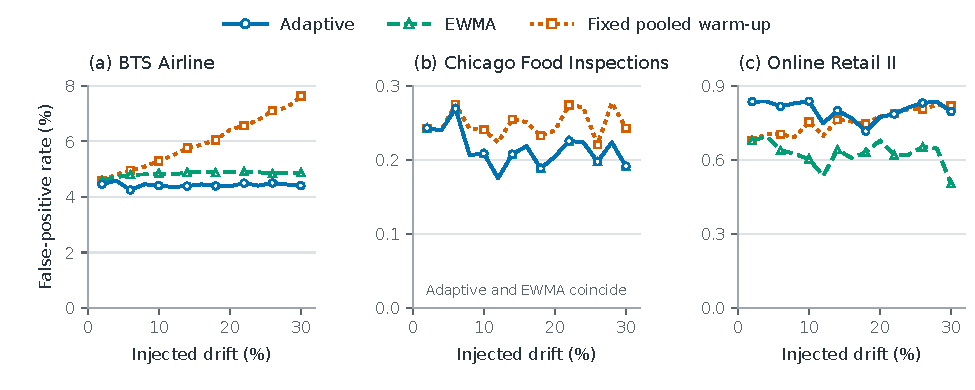
\includegraphics[width=\linewidth]{figures/h1a_fpr_over_time.pdf}
\caption{False-positive rate under gradual legitimate drift (scenario B). Each point pools false-positive and valid-record counts over ten test seeds at an evaluated batch; injected drift increases from 2\% at $B_6$ to 30\% at $B_{20}$. The panels use different vertical scales. Adaptive and EWMA results coincide on Chicago. Numerical coordinate bounds remain fixed in that dataset; its policy difference comes from category handling.}
\Description{Three line charts compare adaptive, EWMA and fixed pooled-warm-up rules. Fixed-rule false positives increase markedly under flight-data drift, while adaptive and EWMA rules remain lower. Chicago rates are much smaller and the adaptive and EWMA lines coincide. On retail data fixed and adaptive rates remain close, with EWMA lower. All panels begin at zero but have dataset-specific vertical scales.}
\label{fig:fpr}
\end{figure}

\begin{table}[t]
\caption{False-positive rate (\%) and recall of every threshold method under gradual drift (scenario B). Deequ ``default rules'' suggests constraints on the warm-up as observed; ``best case'' uses a warm-up without erroneous records and extended rules. ``Failed constraints'' counts records that violate a constraint that failed on the batch; ``any violation'' counts records that violate any suggested constraint.}
\label{tab:h1a:methods}
\footnotesize
\begin{tabular}{@{}lrrrrrr@{}}
\toprule
& \multicolumn{2}{c}{BTS} & \multicolumn{2}{c}{Chicago} & \multicolumn{2}{c}{Retail} \\
\cmidrule(lr){2-3}\cmidrule(lr){4-5}\cmidrule(l){6-7}
Method & FPR & Recall & FPR & Recall & FPR & Recall \\
\midrule
\inputtable{tables/h1a_methods.tex}
\bottomrule
\end{tabular}
\end{table}

Table~\ref{tab:h1a:methods} also shows why calibration and comparator configuration matter. Textbook robust multipliers flagged 7.6--28\% of valid flight and retail records. After warm-up calibration, rolling robust rules and EWMA came within approximately 0.4--0.5 pp of adaptive FPR on BTS. Much of the improvement over fixed bounds is therefore also obtained by these recent-history alternatives. Deequ's default suggestions on observed warm-up were tolerance-based completeness constraints, detecting the missing-value quarter of injected errors. Its favourable extended configuration detected 53--70\% of errors, but generated constraints failed on every erroneous evaluated batch and flagged roughly a fifth of valid Chicago and Retail records. These findings concern the suggested constraint sets and attribution modes tested here, not the full range of rules a practitioner could implement in Deequ.

\subsection{H1b: Separating Drift from Degradation}
\label{sec:res:h1b}

Table~\ref{tab:h1b} reports the four-class macro-F1 of every batch labeller over 600 batches per dataset (ten seeds, four scenarios, fifteen batches).

\begin{table}[t]
\caption{Four-class batch labelling in scenarios A--D. F1 is pooled macro-F1; Drift and Degr.\ are class recalls. A circle marks a comparison whose paired interval does not establish superiority of the proposed classifier. This is not an equivalence test; paired uncertainty is calculated from per-seed macro-F1.}
\label{tab:h1b}
\footnotesize
\begin{tabular}{@{}lrrrrrrrrr@{}}
\toprule
& \multicolumn{3}{c}{BTS} & \multicolumn{3}{c}{Chicago} & \multicolumn{3}{c}{Retail} \\
\cmidrule(lr){2-4}\cmidrule(lr){5-7}\cmidrule(l){8-10}
Labeller & F1 & Drift & Degr. & F1 & Drift & Degr. & F1 & Drift & Degr. \\
\midrule
\inputtable{tables/h1b.tex}
\bottomrule
\end{tabular}
\end{table}

The proposed classifier reached pooled macro-F1 of 0.966, 0.955 and 0.947 on BTS, Chicago and Retail. On BTS, it exceeded all evaluated comparators. Its effect-floor variant was closest, with a mean per-seed difference of approximately $+0.04$; calibrated TFDV followed at $+0.15$ $[0.08,0.21]$, and gated EWMA at $+0.23$ $[0.19,0.27]$. The gated fixed classifier recognised degradation but had drift-class recall of only 0.09: its fixed ranges converted valid distribution movement into higher failure rates, labelling 89\% of pure-drift batches as degraded. Adaptive thresholds lowered this share to 2.5\%, linking the batch-label improvement to their reduction of drift-induced record failures.

The same attribution does not hold on the other datasets. Chicago's gated fixed, EWMA and adaptive variants produced identical results. On Retail, gated fixed thresholds had a higher point score, 0.956 versus 0.947; the mean per-seed difference was $-0.009$ $[-0.027,+0.003]$. This establishes no detected adaptive advantage, rather than equality of the methods. Removing the gate, however, lowered pooled macro-F1 to 0.658, 0.668 and 0.720 across the three datasets. Without filtering, erroneous records changed the drift score and caused degradation-only batches to be labelled drift with degradation. The consistent contributor is therefore the gated drift evidence, with threshold adaptation adding a dataset-dependent benefit.

The documented Deequ and TFDV configurations scored below the proposed classifier on this four-state task. TFDV against the previous batch assigned almost all batches the same label; cumulative-history Deequ detected few anomalies, giving macro-F1 of approximately 0.10--0.23. Warm-up calibration raised TFDV to 0.82--0.90 and Deequ to 0.36--0.61. The AVH-inspired baseline scored about 0.28 when updated from all history and 0.43--0.56 when updated only from alarm-free batches. Its restricted metric library and the difference between anomalous-partition detection and persistent-state classification limit direct comparison with published AVH. The proposed classifier identified degradation in its onset batch in every evaluated run, and mean drift delay was 0.3, 0.9 and 0.0 batches. These controlled detection delays should not be read as guarantees for unlabelled operational incidents.

Adding a minimum drift-effect size excluded small injected shifts and lowered macro-F1 to 0.71--0.93 under labels that count every positive injected drift as drift. That reduction reflects the distinction between detecting any constructed change and prioritising operationally meaningful changes. The temporal replay examines the same trade-off without changing the primary controlled labels (Section~\ref{sec:res:replay}).

\subsection{H2a: Coverage of Validated LLM Rules}
\label{sec:res:h2a}

Table~\ref{tab:h2a} reports the recall of domain-impossible values (semantic recall) and the FPR of each rule configuration under drift (scenario S2); scenario S1 gave the same picture.

\begin{table}[t]
\caption{Semantic recall and FPR (\%) in scenario S2. Model results average five generations and ten seeds. Admitted rules pass historical screening; dictionary-only rules are authored by a third model, not human experts. Near-perfect semantic recall belongs to fixed statistical rules combined with LLM rules.}
\label{tab:h2a}
\footnotesize
\begin{tabular}{@{}lrrrrrr@{}}
\toprule
& \multicolumn{2}{c}{BTS} & \multicolumn{2}{c}{Chicago} & \multicolumn{2}{c}{Retail} \\
\cmidrule(lr){2-3}\cmidrule(lr){4-5}\cmidrule(l){6-7}
Rules & Sem.\ recall & FPR & Sem.\ recall & FPR & Sem.\ recall & FPR \\
\midrule
\inputtable{tables/h2a.tex}
\bottomrule
\end{tabular}
\end{table}

The two rule sources cover different error families. Fixed statistical rules detected invalid codes absent from warm-up, but only 3--6\% of impossible numerical flight values and less than 1\% of non-positive quantities or negative prices in Retail. Admitted LLM rules supplied restrictions such as non-negative taxi time and price, detecting the impossible numbers but missing many well-formed invalid codes in open domains. Fixed statistical rules combined with admitted LLM rules reached semantic recall of 0.996--1.00 on every dataset with either model. The gain over fixed statistical rules was $+0.48$ $[0.47,0.48]$ on BTS and $+0.49$ $[0.49,0.50]$ on Retail. Chicago was already at 1.00 because its injected semantic violations were categorical. The primary-model FPR increase was at most 0.01 pp, within the 0.5 pp tolerance. H2a is thus supported on BTS and Retail; Chicago's ceiling prevents an incremental-coverage conclusion.

Adaptive statistical rules detected only 0.07--0.13 of the same domain-impossible subset. Invalid codes recurred at 1\% in every batch and entered the allowed set after two batches. Adding LLM rules restored impossible-number detection, but not the open-domain codes; adaptive+LLM semantic recall remained 0.62--0.75. The near-perfect fixed+LLM result and the weaker adaptive+LLM result must therefore remain distinct. The separate guard experiment in Section~\ref{sec:res:h2b} investigates the category mechanism, but does not supply an integrated-system result for this configuration.

\paragraph{Admission.} Every naturally generated LLM candidate passed admission in the test runs: no candidate was malformed, exceeded the historical flag-rate ceiling or was logically implied by a kept rule. No admitted candidate exceeded 0.5\% FPR on valid evaluation records. This establishes historical and held-out compatibility for the observed candidates, not the frequency with which admission would remove harmful proposals in general. The filter acted on the dictionary-only model-authored comparison rules. Before admission they flagged 10.8\% of valid BTS records, 22.1\% of Chicago records and 0.9\% of Retail records under drift. Faulty patterns rejected carriers B6 and 9E, apostrophes in facility types and stock code POST; a category list omitted three valid inspection results. After admission their FPR was 0.00--0.03\%. Under the study's held-out-FPR criterion, no harmful comparison rule was retained and no compatible one rejected. This operational criterion is narrower than semantic correctness.

A controlled stress test supplied cases absent from the natural candidate sets: malformed, too-strict, wrong, subtly too-strict, sound, vacuous and redundant rules. All malformed rules were rejected, sound rules accepted, and vacuous or redundant rules dropped. Wrong rules initially flagging almost every valid record were rejected, dropped or relaxed; surviving rules produced 0.3--2.1 false positives per 10,000 valid records. Too-strict rules fell from 2,770--5,351 false positives per 10,000 to 1.0--3.8. This isolates the admission mechanism's filtering effect. It does not imply that relaxation preserves every useful domain distinction or estimate the natural rate of LLM rule errors.

\paragraph{Stability and cost.} Generations showed high value-level agreement on sampled and synthetic probes: 98.5--99.4\% within a model and 98.4--99.0\% between models. The primary model proposed 10.6--15.4 rules per generation and the secondary 7.8--18.0. Agreement describes the probe set, not comprehensive logical equivalence of rule suites. The thirty controlled generations have estimated cost US\$2.14, using configured prices and corrected input-token estimates as described in Section~\ref{sec:design}. Costs of per-value category judgements are reported separately.

\subsection{H2b: Guarding Category Admission}
\label{sec:res:h2b}

Table~\ref{tab:h2b} reports the share of valid and invalid novel values that each policy admitted (Figure~\ref{fig:guard} shows the same data).

\begin{table}[t]
\caption{Share of novel category values admitted, valid / invalid, over ten seeds and both novelty scenarios. Ideal: valid 1, invalid 0. Distinct values: BTS 6 valid and 6 invalid, Chicago 4 and 4, Retail 2 and 2.}
\label{tab:h2b}
\footnotesize
\begin{tabular}{@{}lrrrrrr@{}}
\toprule
& \multicolumn{2}{c}{BTS} & \multicolumn{2}{c}{Chicago} & \multicolumn{2}{c}{Retail} \\
\cmidrule(lr){2-3}\cmidrule(lr){4-5}\cmidrule(l){6-7}
Admission policy & Valid & Invalid & Valid & Invalid & Valid & Invalid \\
\midrule
\inputtable{tables/h2b.tex}
\bottomrule
\end{tabular}
\end{table}

\begin{figure}[t]
\centering
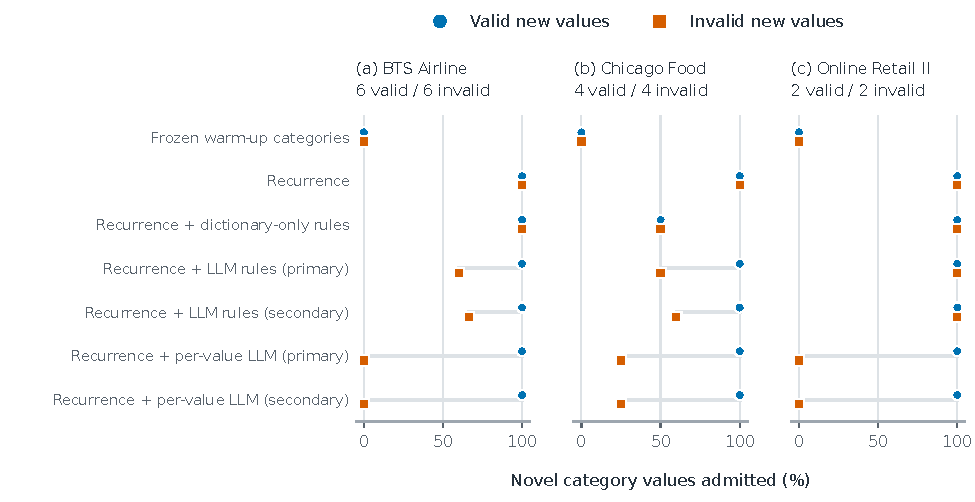
\includegraphics[width=\linewidth]{figures/h2b_category_guard.pdf}
\caption{Percentage of valid (circles) and invalid (squares) novel category values admitted by each policy, over ten test seeds and both novelty scenarios. Primary and secondary LLM policies are shown separately; the LLM-constraint rows also average the five rule generations. The ideal policy admits valid values and rejects invalid values. There are only 24 distinct values: BTS six valid and six invalid, Chicago four and four, and Retail two and two. Seed replays do not add independent semantic cases.}
\Description{Three dot-chart panels show admission percentages for seven policy/model rows. Frozen categories admit no novel values; recurrence admits all valid and invalid values. Constraint guards admit many invalid values. Per-value LLM checks admit all valid values and reject all invalid values on BTS and Retail, but admit one quarter of the invalid Chicago values. The two models have separate rows.}
\label{fig:guard}
\end{figure}

Frozen categories and unrestricted recurrence define the two extremes: the former rejects every novel value, while the latter admits every valid and invalid novel value after two batches. Constraint guards help only when their conditions separate valid membership from plausible syntax. Most open-domain LLM rules are patterns; an invalid airport code can still contain three upper-case letters. LLM-constraint guards therefore admitted 50--100\% of invalid values, recorded as unresolved where only pattern compatibility was established. Dictionary-only constraints did no better on invalid values and excluded half of Chicago's valid novelty. These outcomes distinguish syntactic admissibility from membership in a particular domain.

The per-value policy admitted all twelve valid values and rejected eleven of twelve invalid values. Both models accepted the undocumented result \emph{Not Inspected}, while rejecting \emph{Pass Conditional}, \emph{Restuarant} and \emph{Bakkery}. Their verdicts agreed on all 24 cases. H2b is supported for this per-value policy on the selected cases, but repeated seeds do not create independent semantic test sets. Values already in warm-up bypass the query, and unsure or missing verdicts revert to recurrence. Candidate verdicts were cached before replay without injected labels; the experiment does not measure live online query latency. Across development and test runs, 362 queries per model yielded token-based cost estimates of US\$2.34 and US\$3.24.

\subsection{H3: Risk-Based Check Selection}
\label{sec:res:h3}

Table~\ref{tab:h3} reports post-onset recall and the share of checks saved in the eighteen degradation and incident cases.

\begin{table}[t]
\caption{Post-onset recall and checks saved (\%, in parentheses). Bold satisfies H3 using a mean recall of at least 0.90 and positive saving. C/D recall covers all erroneous post-onset records; H1--H4 covers incident-injected records during each incident. Periodic and random schedules target the risk policy's realised standard-check execution rate; finite-run counts can differ.}
\label{tab:h3}
\footnotesize
\begin{tabular}{@{}llrrrrr@{}}
\toprule
Data & Scenario & Risk-based & Periodic & Random & Failure only & Drift only \\
\midrule
\inputtable{tables/h3.tex}
\bottomrule
\end{tabular}
\end{table}

Risk-based selection was useful in 11 of 18 cases, against 4 for cost-matched periodic and 5 for cost-matched random selection. It met the target in every sustained degradation (C, D) and in the sparse-category incident, where the risk of the affected column rose and its checks returned. It failed on sparse duplicates (post-onset recall 0.60 to 0.62), on the short two-batch incident (0.69 to 0.74) and, on the retail data, on the incident with recovery (0.87). In these cases the failure signal of a skipped check could be up to four batches old, and a sparse or short incident gives the risk score little evidence before it ends. A risk score using only the drift component was useful in 13 cases, but it saved at most 3.8\% of checks and almost nothing (0 to 0.1\%) in scenario D, where drift kept the drifting columns at high risk. A score using only failures saved more and was useful in 8 cases. The savings of risk-based selection were small throughout: 2.1 to 11.3\% of executed checks across all 24 dataset and scenario combinations, and 1.2 to 8.8\% of bytes scanned.

\begin{table}[t]
\caption{Phase timing in scenario A, milliseconds per batch: median across five repetitions of the mean over fifteen evaluated batches, first test seed. Reuse applies to execution and drift gating. Other combines read, adapt, select, label and persist. Component medians need not sum exactly to the independently summarised total.}
\label{tab:runtime}
\footnotesize
\begin{tabular}{@{}lrrrrr@{}}
\toprule
Configuration & Profile & Drift & Execute & Other & Total \\
\midrule
\inputtable{tables/runtime.tex}
\bottomrule
\end{tabular}
\end{table}

Phase measurements distinguish check savings from end-to-end savings (Table~\ref{tab:runtime}). Without reuse, profiling and drift account for 58--67\% of total time and execution for 26--31\%. Risk reduces median repetition-level mean time from 60.3 to 54.1 ms/batch on BTS, 18.5 to 16.9 on Chicago and 65.6 to 61.4 on Retail. When profile statistics and masks are reused, execution takes approximately 2.2--6.4 ms/batch; all-check/risk totals are 49.9/49.6, 14.9/14.9 and 38.0/38.1 ms/batch. There is then no material end-to-end gain from selection. Reuse also reduces work in the drift gate, so its effect is not confined to the Execute column. These corrected per-batch values divide the recorded fifteen-batch totals by fifteen; relative configuration comparisons are unaffected by the unit correction.

\subsection{Ablation}
\label{sec:res:ablation}

Table~\ref{tab:ablation} gives balanced main effects from the eight-configuration design, averaging over the other two factors and scenarios A--D, S1 and S2. They summarise how each component changes the tested system on average; they are not the effect of a single selected deployment. No per-value category guard is included, and the main-effect table does not provide confidence intervals for effects or interactions.

\begin{table}[t]
\caption{Main effects in the $2 \times 2 \times 2$ ablation. Recall, semantic recall and macro-F1 in absolute units, FPR in pp, bytes scanned in percent of the dataset mean.}
\label{tab:ablation}
\footnotesize
\begin{tabular}{@{}llrrrrr@{}}
\toprule
Factor & Data & Recall & Sem.\ recall & FPR & Macro-F1 & Bytes \\
\midrule
\inputtable{tables/ablation.tex}
\bottomrule
\end{tabular}
\end{table}

Adaptation lowered record recall on all three datasets and semantic recall by 0.33--0.58, consistent with category absorption in Section~\ref{sec:res:h2a}. Its macro-F1 main effect was $+0.10$ on BTS, $-0.06$ on Chicago and $-0.16$ on Retail. Admitted LLM rules increased record recall, semantic recall and macro-F1 without a material FPR change, but added text-pattern scans. Their byte main-effect difference was 30--38\% of the dataset mean estimated bytes. Selection reduced bytes by 1.4--3.9\% of that same mean while lowering record recall by 5--6 points. These denominators differ from percentage change relative to a no-LLM or all-check configuration. The trade-offs reinforce the need to attribute effects to the particular combination being evaluated.

\subsection{External Validity}
\label{sec:ext}

\paragraph{Benchmarks with real errors.} Table~\ref{tab:external} reports the results on the Tax and Beers benchmarks.

\begin{table}[t]
\caption{Error-labelled benchmarks. Tax: record recall, FPR (\%), and cell recall/precision over checkable columns, which contain about 67.7\% of all erroneous cells. Beers: cell metrics, because every evaluated record is erroneous and record FPR is undefined.}
\label{tab:external}
\footnotesize
\begin{tabular}{@{}lrrrrrr@{}}
\toprule
& \multicolumn{4}{c}{Tax} & \multicolumn{2}{c}{Beers} \\
\cmidrule(lr){2-5}\cmidrule(l){6-7}
Method & Recall & FPR & Cell rec. & Cell prec. & Cell rec. & Cell prec. \\
\midrule
\inputtable{tables/external.tex}
\bottomrule
\end{tabular}
\end{table}

Single-column rules detected about 20\% of erroneous Tax cells within checkable columns under every threshold policy. Cross-column dependencies learned from warm-up raised this recall to 0.908 and record recall from 0.153 to 0.626, while FPR moved from 3.06\% to 3.12\%. The primary LLM's proposed dependency structure reached the same record recall and checkable-column cell recall, but cell precision was lower: 0.130 versus 0.175 for dependencies learned without an LLM. The secondary model's structure reached cell recall 0.690. Adding primary single-column LLM rules to the adaptive suite reached only 0.294. These results support the relevance of relationships between fields, rather than an LLM-specific advantage on Tax.

Checkable columns contain approximately 67.7\% of all Tax error cells. Consequently the 0.908 result corresponds to 12,257 detected cells out of 19,944 total error cells, or about 61.5\% overall coverage. Cross-column rules flag participating tuple cells, which contributes to low precision. On Beers, cell recall is approximately 0.996--0.999 across methods; cell precision is 0.650 for first-batch fixed thresholds and 0.853--0.867 for pooled, rolling and adaptive policies. High recall on this table is therefore less discriminating than precision. Both tables test transfer to dirty/clean benchmarks under shuffled replay, not naturally evolving incidents.

\paragraph{Chronological replay.}
\label{sec:res:replay}
Figure~\ref{fig:replay} shows the share of flagged records and the labels over 196 months of raw Chicago inspections. Against a rolling reference of the previous five months, the monitor labelled 143 months as drift, 10 as drift with degradation, none as degradation alone, and 43 as stable. The procedure change of July 2018 was labelled drift in the result column in July, August, September and October 2018 and was never labelled degradation. The ten degradation months coincided with bursts of missing facility types in 2012 and 2014, missing risk categories in 2010, and spikes of unusual result and facility-type values in 2015 and 2017.

\begin{figure}[t]
\centering
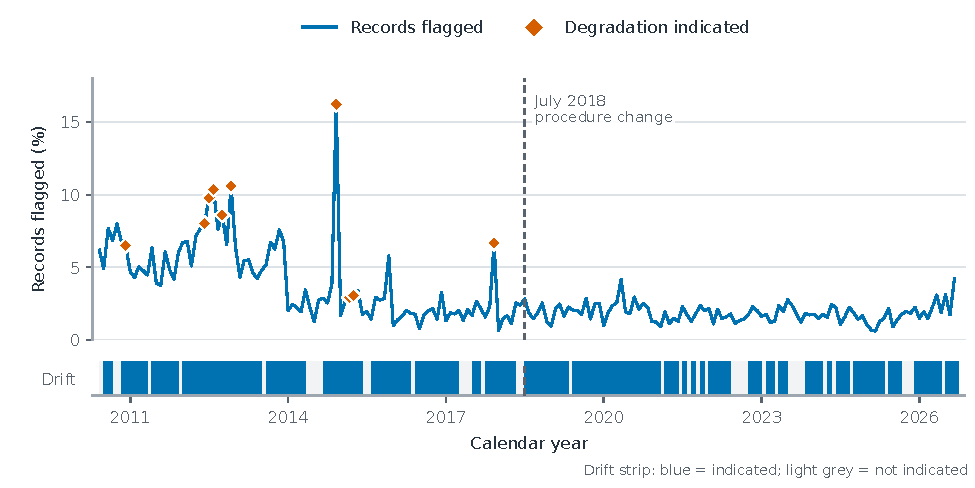
\includegraphics[width=\linewidth]{figures/chicago_temporal.pdf}
\caption{Chronological replay of raw Chicago food-inspection records using the rolling drift reference and all checks, over 196 evaluated months (June 2010--September 2026). The upper panel shows the percentage of flagged records; diamonds identify months labelled degradation, including drift with degradation. The lower strip shows months with a drift indication in blue and other months in light grey. The dashed line marks the documented procedure change on 1 July 2018. These are monitor outputs, not exhaustive ground-truth labels for all changes.}
\Description{A monthly line chart shows the flagged-record percentage from 2010 to 2026, with ten diamond markers at degradation indications. A lower monthly strip distinguishes drift indications from other months. A dashed vertical line marks the July 2018 inspection-procedure change. The flagged percentage is generally higher before 2015 and mostly lower afterward, while drift is indicated in many months.}
\label{fig:replay}
\end{figure}

The rolling-reference monitor labels most months as drift. Monthly batches average about 1,580 records, so comparatively small changes in category mixtures can exceed thresholds calibrated on five initial months. The minimum-effect-size variant reduces drift-only months from 143 to 74 while retaining the July 2018 transition. Against the original warm-up, 195 of 196 months are labelled drift. This demonstrates the operational importance of reference choice and effect size, rather than establishing that all such alarms identify meaningful change.

Some alarms can be assessed under the stated schema and domain policy without injected labels. Missing monitored values are errors under that policy. Risk and result values that remain inside their documented domains are admissible, so category-list alarms on those values are false alarms under domain membership; this does not establish the factual correctness of each inspection record. Facility Type has 3,276 alarms across 433 distinct values. Human adjudication remains outstanding for all of them. A provisional triage combines deterministic format-variant rules (40 values, 573 alarms) with model suggestions for the remaining values, assigning approximately 93\% of alarms to non-error, 3.5\% to error and 3.5\% to unclear. These are suggestions for review, not human-validated precision. Overlapping check-record alarms are not summed as distinct erroneous records.

\subsection{Sensitivity Analysis}
\label{sec:res:sens}

Five claims were re-checked while one setting at a time was changed and everything else stayed frozen (Table~\ref{tab:sens}). Five dials were prespecified before freezing: the error rate (1 to 20\%), outlier severity, the drift and degradation multiplier $z$ (2 to 4), the risk weights (each weight multiplied by 0, 0.5 or 2, and equal weights) and the risk thresholds. Three dials were added after freezing and are reported as post-hoc: the range multiplier $k$ (2.5 to 4), the history window (3 to 10 batches) and the drift budget $\alpha$ (0.01 to 0.20).

\begin{table}[t]
\caption{Sensitivity criterion counts on their assigned scenario subsets, ten test seeds per setting. H1a uses A/B, not contamination F1/F2. C1/C2 use paired interval criteria; C3--C5 are descriptive point comparisons, and C5 concerns sustained degradation C/D.}
\label{tab:sens}
\footnotesize
\begin{tabular}{@{}lrrr@{}}
\toprule
Claim & BTS & Chicago & Retail \\
\midrule
\inputtable{tables/sensitivity.tex}
\bottomrule
\end{tabular}
\end{table}

BTS and Chicago meet every listed criterion over the settings and scenario subsets assigned to it. This does not overturn their persistent-contamination failures, because the H1a sensitivity grid uses A/B rather than F1/F2. On Retail, the FPR-related and comparative macro-F1 criteria fail in all tested settings, including default settings; these failures are therefore stable within this sensitivity grid rather than dependent on one parameter choice. Two other verdicts vary: mild-outlier recall non-inferiority on Retail, whose difference is $+2.4$ pp with a lower bound of $-1.45$ pp, and usefulness of risk selection at moderate-risk threshold 0.10. One-at-a-time sensitivity describes these tested perturbations; it does not establish robustness to all joint parameter changes.

\subsection{Summary of Verdicts}

Table~\ref{tab:verdicts} collects the decisions without pooling unlike datasets. It distinguishes failure to meet a prespecified criterion, identical observed predictions, absence of detected superiority, ceiling-limited coverage and point-estimate scheduling usefulness. These distinctions are necessary to connect the evidence back to RQ1--RQ3 without extending the hypotheses after seeing the outcomes.

\begin{table}[t]
\caption{Summary of hypothesis verdicts on the confirmatory test run.}
\label{tab:verdicts}
\footnotesize
\begin{tabularx}{\linewidth}{@{}lXXX@{}}
\toprule
Hypothesis & BTS & Chicago & Retail \\
\midrule
H1a lower FPR, recall non-inferior & Supported in 6 of 9 scenarios; fails under mild errors without drift and under contamination & Supported in 9 of 9; margin 0.03 pp, from the category policy & Not supported (0 of 9); lower FPR not established, recall often higher \\
H1b four-class labelling & Supported; better than all comparators & Identical to gated fixed and EWMA on these runs & No detected advantage over gated fixed or EWMA \\
H2a validated LLM rules add coverage & Supported ($+0.48$) & Undecidable (ceiling at 1.00) & Supported ($+0.49$) \\
H2b guarded admission & Supported for per-value check; not for list or pattern constraints & Partly: one of four invalid values admitted by per-value check & Supported for per-value check \\
H3 risk-based selection useful & 4 of 6 cases (mean criterion) & 4 of 6 cases (mean criterion) & 3 of 6 cases (mean criterion) \\
\bottomrule
\end{tabularx}
\end{table}

\section{Discussion}
\label{sec:discussion}

\subsection{What the Evidence Supports}

The evaluation addresses the three objectives through distinct but interacting components: maintaining record-level detection under legitimate change, interpreting batch changes, and allocating validation work. The results support conditional benefits rather than uniform superiority of the complete adaptive configuration.

\paragraph{The gated drift signal carries the batch labels.} Removing the gate reduces macro-F1 by roughly 0.23--0.31 across all datasets. Filtering records that fail basic checks keeps some error-induced distribution movement out of the drift estimate, allowing failure evidence and distribution evidence to play different roles. On Chicago, fixed or EWMA failure thresholds behind the same gate produce identical predictions to adaptive thresholds. On Retail, their point estimates are higher and the paired analysis establishes no adaptive advantage. Adaptation adds most clearly on BTS, where fixed bounds otherwise label 89\% of pure-drift batches as degraded. Thus the strong four-way scores should be attributed to the combination of signals and their calibration, with adaptation's incremental contribution assessed separately. The gate is still heuristic: excluded records may include valid novelty, and undetected errors may remain in the retained data.

\paragraph{Adaptation pays off where drift moves valid values across fixed bounds.} In BTS, a changing delay or taxi-time distribution increasingly crosses fixed limits; adjusting location and scale removes much of this additional false alarming. In Retail, broad fixed ranges already accommodate the tested multiplicative change. Adaptation then trades a small FPR increase for higher recall, which does not satisfy an FPR-reduction hypothesis. Chicago is different again: its numerical columns retain physical bounds, and the improvement comes from category recurrence. These cases show why policy performance depends on both the data distribution and the monitored domain. In practice, a historical replay can establish whether fixed limits produce growing false alarms under expected change before numerical adaptation is selected.

\paragraph{Adaptation absorbs persistent errors.} Repeated observations are evidence of frequency, not independent evidence of validity. The tested numerical policy loses up to 29.06 points of recall under persistent taxi-out contamination. The categorical policy admits recurring invalid codes, reducing statistical semantic recall from approximately 0.51--1.00 under fixed rules to 0.07--0.13 under adaptive rules. All profiles enter history, so the drift gate does not protect numerical learning from suspect batches. Fixed domain constraints and guarded category admission can retain distinctions that recurrence and broad ranges lose. Their evidence must nevertheless remain configuration-specific: fixed+LLM rules attain the highest injected semantic recall, while the per-value guard is evaluated separately on only 24 distinct values. No result here establishes a fully integrated guarded monitor's performance.

The connection with poisoning research~\cite{Biggio2012,Steinhardt2017} is an interpretation of the same learning mechanism, not an evaluated adversarial threat model. A persistent invalid value can become statistically normal whether it originates in an accidental mapping error or deliberate manipulation. The present evidence supports limiting what history may authorise, without claiming an evaluated security defence.

\paragraph{Selective execution is limited by monitoring overhead.} Risk selection meets the point-estimate usefulness criterion more often than matched periodic or random schedules, showing that the observed risk signals help allocate some checks. Savings remain modest because basic checks always run and profile and drift work continue on every batch. After reuse, skipping optional checks produces no material end-to-end timing benefit in these workloads. Conversely, the ablation shows that text-pattern rules add scanning work: their main-effect byte difference is 30--38\% of the dataset mean. Selectivity is therefore most relevant when optional checks account for a substantial part of total cost, a condition that must be measured rather than inferred from check counts. Sparse and short incidents expose the opposing risk: skipping a check also withholds the evidence that would raise its priority.

\subsection{Implications for Practice}

Four implications follow directly from the evaluated setting. First, retain separate distribution-change and check-failure evidence. A single unusualness score cannot identify why a batch changed, and an operational label should remain interpretable through the contributing columns and checks. Second, calibrate drift thresholds against the available warm-up variability and verify the resulting stable-batch behaviour. The resampling procedure improved development calibration here, but five historical batches do not justify a general finite-sample guarantee.

Third, distinguish a data contract from a learned expectation. Physical bounds and documented domain membership require independent justification; repeated presence or compatibility with a pattern is insufficient. Historical screening remains useful for rejecting overly restrictive proposals, but relaxing a semantic rule to observed values can also weaken its intended meaning. The dictionary-only model rules demonstrate the value of screening, while their unequal information access prevents a comparison with human expert quality.

Fourth, measure total monitoring cost as well as work avoided. Reuse existing profile statistics before interpreting skipped-check savings as a runtime benefit. Report incident recall and observation staleness alongside the execution rate, because a schedule can save checks while missing the short events that matter operationally. These recommendations apply to the evaluated batch setting; deployment-specific tolerance for missed errors and alarms remains a policy decision.

\subsection{Threats to Validity}

\paragraph{Internal validity.} Development and test pools contain disjoint records and use separate seeds, but derive from the same three datasets. Changes to calibration, retention of known categories and selective-execution gating were made during development and documented before the internal freeze. Three later sensitivity dials are explicitly post-hoc. Manifests identify the tested code and settings, but do not provide independent public preregistration. Comparator implementation remains an author-controlled factor. In particular, the AVH-inspired baseline omits the original optimiser, and default versus calibrated tool configurations should not be interpreted as a tool-wide ranking.

\paragraph{Construct validity.} Injected labels isolate mechanisms but simplify natural error processes. A positive injected drift level defines drift even when the change is operationally small; degradation denotes an increased error rate rather than an independently logged business incident. Rule failures provide observable evidence, not a direct census of all errors. Current-batch adaptation also uses information unavailable to a strictly predictive policy. Record FPR does not fully express batch alert burden. Logical bytes touched approximate implementation work rather than measured cloud I/O, and all timing comes from one seed and one machine.

\paragraph{External validity.} Three domains, two dirty/clean tables and one natural timeline do not represent all pipelines. LLM findings depend on the specific endpoints, prompts and selected violations. The dictionary-only baseline is another model, not a domain expert. Category guarding tests twelve valid and twelve invalid distinct values, repeated across seeds; it does not cover initially present invalid categories, which bypass the per-value check. Tax cell recall is conditional on checkable columns, and the strongest cross-column configuration has low cell precision. Chicago's known procedure change provides one interpretable event, while all 3,276 Facility Type alarms still require independent human adjudication.

\paragraph{Conclusion validity.} Ten seed clusters provide uncertainty about replay variation conditional on the source datasets. Bootstrap intervals can be coarse, and pooled macro-F1 differs from the seed-mean estimand used for its paired comparison. Primary H1a decisions are per scenario, not a study-wide familywise guarantee. The separate secondary Holm reporting correction does not remedy the approximate calibration of the original bootstrap sign-tail $p$-values. Descriptive sensitivity criteria, H3 point-estimate passes and non-significant comparisons should not be read as inferential guarantees. Finally, statistical differences may be operationally minor: Chicago's approximately 0.03 pp FPR reduction is clear but small, whereas the BTS contamination recall losses are substantial.

\section{Conclusion}
\label{sec:conclusion}

This article evaluated adaptive and cost-aware data quality monitoring for evolving batch pipelines. The monitor combines numerical adaptation, four-way batch labelling, historical admission of LLM-proposed rules, category-admission guards and risk-based check selection. Its evaluation addresses the three research questions using prespecified criteria, compares components with calibrated alternatives and configured tools, and supplements controlled injection with dirty/clean benchmarks and chronological replay.

The results identify where each component contributes. Four-way macro-F1 reaches 0.947--0.966, but fixed thresholds behind the same gated drift signal perform identically on Chicago and show no detected disadvantage on Retail. Numerical adaptation contributes most clearly on BTS, reducing drift-induced false alarms, while the small Chicago benefit comes from category policy. Retail does not meet the lower-FPR hypothesis. Persistent contamination and invalid-category recurrence demonstrate that adaptive expectations can also weaken error detection.

Domain and statistical rules are complementary. Fixed statistical rules with admitted LLM rules reach semantic recall of 0.996--1.00 on the selected injected violations with at most a 0.01 pp primary-model FPR increase. This result does not describe the adaptive combination, which remains vulnerable to recurring invalid codes. A separate per-value policy admits all twelve valid novel values and rejects eleven of twelve invalid values. Tax further shows that cross-column relationships matter: learned dependencies raise cell recall within checkable columns from about 0.20 to 0.91, with the primary LLM's structure matching rather than exceeding that record recall.

Risk-based selection is useful in eleven of eighteen degradation/incident cases by the specified mean-recall criterion, but saves only about 2--11\% of checks. Profiling and drift work dominate total cost, and selection adds no material timing benefit after profile reuse in the measured workloads. The chronological Chicago replay labels the documented July 2018 procedure change as drift without degradation, while also revealing substantial alert burden and incomplete human ground truth.

The limitations identify four remaining tasks within the existing research scope. Human adjudication of replay alarms and expert-authored comparison rules would strengthen semantic interpretation. Pipelines with logged natural incidents would test the injected definition of degradation. Improving the efficiency of profiling and drift calculation would address the dominant observed cost. Finally, evaluating cross-column rules within the adaptive chronological loop would extend the existing benchmark analysis to the monitored setting. These are follow-up validation needs, not completed results.

The central implication is that adaptation and validation must remain distinguishable. A monitor should follow legitimate changes while preserving independently justified constraints on valid data, and its detection and cost benefits should be assessed for the exact configuration used.

\section*{Data and Code Availability}
The three source datasets and two benchmark tables are public~\cite{BTS2024,Chen2019,Chicago2026,Mahdavi2019}. The research artifact contains the monitoring implementation, experiment harness, frozen configurations, cached responses, run manifests and result tables. These materials are intended for public release with the final article. A public archival repository identifier is not specified in this version.


\begin{acks}
The rule-generation step of the method calls large language models (Claude Opus 5.5 and GPT-6 Astra through Amazon Bedrock), and the manual comparison rules were written by a third model (Llama 4 Maverick), as described in Sections~\ref{sec:method} and~\ref{sec:design}. Claude (Anthropic) was also used to assist with the experiment code and with drafting this manuscript. Codex was used to assist with language revision and figure-generation code for the present manuscript. The authors are responsible for verifying the code, experimental provenance, references, and final text.
\end{acks}

\bibliographystyle{ACM-Reference-Format}
\bibliography{references}

\end{document}
